%%####################################################################
%    Copyright @ 2007-2017 Andreas Frie� (Friess)
%    Permission is granted to copy, distribute and/or modify this document
%    under the terms of the GNU Free Documentation License, Version 1.2
%    or any later version published by the Free Software Foundation;
%    with no Invariant Sections, no Front-Cover Texts, and no Back-Cover Texts.
%    A copy of the license is included in the section entitled ``GNU
%    Free Documentation License''.
%%####################################################################
% Created: 21.08.2007
%%####################################################################
%% Artikelvorlage unter Verwendung der Artikelklasse des KOMA-Script %%
%% Basierend auf einer TeXNicCenter-Vorlage von Mark M�ller          %%
%%%%%%%%%%%%%%%%%%%%%%%%%%%%%%%%%%%%%%%%%%%%%%%%%%%%%%%%%%%%%%%%%%%%%%%

\documentclass[
titlepage,						% Titelei auf eigener Seite
]
{scrreprt}
%%{scrartcl}

\ifpdfoutput{
  % PDF wird genutzt
  \usepackage[activate]{pdfcprot}				
	\usepackage[pdftex]{graphicx} %%Grafiken in pdfLaTeX
  \usepackage[pdftex]{graphicx}
  \usepackage[pdftex,
    colorlinks, % Schrift in Farbe, sonst mit Rahmen
    bookmarksnumbered, % Inhaltsverzeichnis mit Numerierung
    bookmarksopen, % offnet das Inhaltsverzeichnis
    pdfstartview=FitH, % startet mit Seitenbreite
    linkcolor=blue, % standard red
    citecolor=blue, % standard green
    urlcolor=magenta, % standard cyan
    filecolor=blue %
    ]{hyperref}
  \pdfinfo{
    /Title (LazInfos)
    /Subject (Das Lazarus Beispielbuch)
    /Author (Andreas Frie�)
    /Keywords (LazInfos)
  }
}{
  % Kein PDF
	\usepackage[dvips]{graphicx} %%Grafiken und normales LaTeX
  \usepackage{graphicx}
  \usepackage{hyperref}
}

\usepackage[ngerman]{babel}		
\usepackage[T1]{fontenc}							
\usepackage[latin1]{inputenc}		
\usepackage{picins}
%\usepackage{hyperref}
%\usepackage{times} % Tip von Ovidius, mal ausprobieren

\begin{document}
\ifpdfoutput{
	\DeclareGraphicsExtensions{.pdf,.PDF,.jpg,.JPG,.png,.PNG}
}{
	\DeclareGraphicsExtensions{.eps,.EPS}
}
\setcounter{tocdepth}{3} %Tiefe des Inhaltsverzeichnis

%###############################################
% Umschlag und Titelseite
%###############################################
\pagestyle{empty} %%Keine Kopf-/Fusszeilen auf den ersten Seiten.
\title{LazInfos\\Das Lazarus Beispielbuch}
\author{Andreas Frie�\\Die Community von www.lazarusforum.de}
%\date{}							% falls anderes, als das aktuelle gew�nscht

\maketitle 						% Titelei wird erzeugt

%\begin{abstract}
%This work is licensed under a Creative Commons Attribution-Noncommercial-Share Alike 3.0 License
%\end{abstract}

\pagestyle{headings} %% Kopf-/Fusszeilen aktivieren

%\begin{center}
%\textbf{Version}
%\verb|SVN $LastChangedRevision: 94 $ |
%\end{center}

\begin{quote}
    Copyright (C) 2007-2017 Andreas Frie�.
    Es wird die Erlaubnis gew�hrt, dieses Dokument zu kopieren, zu
    verteilen und/oder zu modifizieren, unter den Bestimmungen der
    GNU Free Documentation License, Version 1.2 oder jede sp�tere
    Version, ver�ffentlicht von der Free Software Foundation; mit
    keinen unver�nderlichen Abschnitten, keinen vorderen
    Umschlagtexten und keinen hinteren Umschlagtexten. Eine Kopie der
    Lizenz ist aufgenommen in den Abschnitt mit dem Titel "GNU Free
    Documentation License".

    Copyright \copyright{}  2007-2017 Andreas Friess
    Permission is granted to copy, distribute and/or modify this document
    under the terms of the GNU Free Documentation License, Version 1.2
    or any later version published by the Free Software Foundation;
    with no Invariant Sections, no Front-Cover Texts, and no Back-Cover Texts.
    A copy of the license is included in the section entitled ``GNU
    Free Documentation License''.
\end{quote}

%###############################################
% Inhaltsverzeichnis
%###############################################
%\section[Inhaltsverzeichnis]{Inhaltsverzeichnis}
\tableofcontents			% Inhaltsverzeichnis

\newpage
%###########################################################
% Einf�hrung, Therorie, ....
%###########################################################
%--------------------------------------------------
% Alles was allgemeine Information ist
%--------------------------------------------------
\chapter[Vorwort]{Vorwort}
\section{Danksagung}
%%####################################################################
%    Copyright @ 2009 Andreas Frieß (Friess)
%    Permission is granted to copy, distribute and/or modify this document
%    under the terms of the GNU Free Documentation License, Version 1.2
%    or any later version published by the Free Software Foundation;
%    with no Invariant Sections, no Front-Cover Texts, and no Back-Cover Texts.
%    A copy of the license is included in the section entitled ``GNU
%    Free Documentation License''.
%%####################################################################
% Created: 01.04.2009
%%####################################################################
\paragraph{Meiner Frau}
Vor allen möchte ich meiner Frau danken. Für ihre schier endlose Geduld mit mir, beim Schreiben dieses Buches.

\paragraph{Mitwirkende}  
carli für das Korrekturlesen,...
%\subsection[Vorwort]{Vorwort}
%\subsection[Grundlagen]{Grundlagen}
\chapter{Grundlagen Datenbank}
\section[Datenbanken]{Datenbanken}
%%####################################################################
%    Copyright @ 2007 Andreas Frieß (Friess)
%    Permission is granted to copy, distribute and/or modify this document
%    under the terms of the GNU Free Documentation License, Version 1.2
%    or any later version published by the Free Software Foundation;
%    with no Invariant Sections, no Front-Cover Texts, and no Back-Cover Texts.
%    A copy of the license is included in the section entitled ``GNU
%    Free Documentation License''.
%%####################################################################
% Created: 22.08.2007
% @cvs($Date: 2007-10-31 21:33:37 +0000 (Wed, 31 Oct 2007) $)
% @cvs($Rev: 55 $)
% @cvs($Author: af0815 $)
% @cvs($URL: file:///svn/p/lazsnippets/code/trunk/dokumentation/LazSnippets/Kapitel/datenbanken/DBEInfuehr1.tex $)
%%####################################################################
\subsection{Einführung in die Datenbanktheorie}
%%####################################################################
Das Folgende Kapitel wendet sich speziell an den Personenkreis der in die Theorie von Datenbanken noch nicht so eingedrungen ist, beziehungsweise dient als Nachschlagwerk für die verschiedenen Begriffe. Man kann also bei entsprechenden Vorwissen die folgenden erklärenden Kapitel überspringen und bei Bedarf nachschlagen.

\subsubsection{Begriffe}
Um Missverständnisse auszuschließen und zu einer gemeinsamen Sprachregelung zu kommen, sollte man die verwendeten Begriffe möglichst genau definieren:

\begin{itemize}
	\item Eine Datenmenge\label{Datenmenge} ist eine Menge von einzelnen Datensätzen. Jeder Datensatz besteht aus mindesten einem Feld. Die Herkunft dieser Datenmenge ist nicht festgelegt.
  \item Eine Tabelle\label{Tabelle} ist als Datenbankbestandteil eine spezielle Ausführung einer Datenmenge. Die Tabelle speichert als physisches vorhandenes Element die Daten.
  \item Eine Abfrage ist eine virtuelle Datenmenge, die den Inhalt von tatsächlich vorhandenen Tabellen in einer frei wählbaren Anordnung abbildet, manchmal auch Projektion genannt.
  \item Eine Datenbank ist eine Zusammenstellung von logisch zusammengehörigen Tabellen.
  \item Ein Datenbankserver verwaltet verschiedene Datenbanken und stellt auch das Management, die Sicherung und andere Verwaltungsdienste zur Verfügung.
\end{itemize}

Wichtige Informationen bei der Entwicklung einer Datenbankanwendung sind das Verhalten der Datenbank bzw. des Datenbankservers selbst.

\subsubsection{Was ist eine Datenbank}

Eine Datenbank ist eine geordnete Sammlung von Daten, die auf irgendeine Weise miteinander in Beziehung stehen.
 
Die ersten Generationen von Datenbanken waren sogenannte File-Systeme. Zuerst auf Band, dann auch auf Festplatten. In diesem Datei-Systemen wurden die Daten nacheinander abgespeichert. Um auf einen bestimmten Datensatz zu zugreifen, muss man an den Anfang der Datei (oder Bandes) gehen und anschließend alle Datensätze durchlaufen, bis man den richtigen gefunden hat. Somit ist auch klar, das ein einfaches sortieren oder einfügen von Daten in eine sortierte Datenmenge enormen Aufwand und Kapazität erfordert hat.
Um diesen Beschränkungen zu entfliehen, (und durch neue, schnellere und größere Festplatten ermöglicht) haben sich aus diesen System die heutigen relationalen oder objektorientierten Datenbanken entwickelt. Die derzeit am meisten verwendeten Datenbanken sind die  relationalen und im weiteren werde ich nur noch diese behandeln.

\subsubsection{Desktop und Client-Server Datenbankarten}
Gerade der Begriff Netzwerkdatenbank ist sehr verwirrend. Wird damit eine Access-Datenbank, die mehrere Benutzer über das Netzwerk verwenden so bezeichnet ? Oder eine Serverbasierende Datenbank? Die folgenden Erklärungen sollten die Begriffe klarer werden lassen.

\paragraph{Stand-Alone Datenbank}
Eine Stand-Alone Datenbank ist eine Desktop-Datenbank, es befinden sich daher die Daten auf dem Arbeitsplatzrechner. Auf die Daten kann immer nur ein Anwender, mit immer nur einem Programm zugreifen. Es ist zwar prinzipiell möglich über ein Netzwerk auf die Datenbankdatei zuzugreifen, aber es kann der eine nur in der Datenbank arbeiten, wenn der andere sein Programm geschlossen hat. Probleme die durch den gleichzeitigen Zugriff entstehen können daher gar nicht auftreten. Bei jeder etwas umfangreicheren Datenbank wird dieses Verhalten zu einem Engpass. Man stelle sich nur vor, der eine Benutzer öffnet die Datenbankdatei und vergisst auf das schließen des Programms. Kein anderer Benutzer kann die Daten in der Zwischenzeit benutzen!

\paragraph{File-Share Datenbank}
Moderne Netzwerke bieten die Möglichkeit, dass mehrer Anwender auf ein und dieselbe Datei zugreifen. Auf diese Weise ist es auch möglich das mehrer Programme auf ein und dieselbe Datenbankdatei zugreifen. Diese Version der Desktop-Datenbank nennt man File-Share Datenbank und damit ist bereits ein echter Mehrbenutzer Betrieb möglich.
Das ganze hat jedoch (unter anderem) einen entscheidenden Nachteil: Die Daten\-verarbeitung erfolgt auf den Arbeitsplatzrechnern. Für Abfragen muss der jeweilige ganze Datenbestand zu den Arbeitsplatzrechnern gebracht werden, dementsprechend hoch ist die Belastung für das Netzwerk. Weiter können auch Störungen am Netzwerk leicht zu Datenverlust bzw. zu inkonsistenz der Datenbeständen führen.

\paragraph{Client-Server Datenbank}
Bei Client-Server Datenbanken hat nur der Daten\-bank\-server selbst direkten Zugriff auf die Dateien des Daten\-bestandes. Anfragen werden somit direkt an den Daten\-bank\-server gestellt, von diesem bearbeitet und die Ergebnisse an den Arbeits\-platz\-rechner zurück\-geliefert. Die Verwaltung beim gleich\-zeitigen Zugriff durch mehrer Arbeits\-platz\-rechner obliegt dem Daten\-bank\-server. Falls eine Verbindung durch eine Störung abbricht, so wird dieses erkannt und die noch nicht kompletten Anfragen verworfen und somit die Konsistenz der Daten erhalten.
Gerade zur File-Share Datenbank können Netzbelastungen drastisch gesenkt werden. Man stelle sich nur vor, das man den größten Wert aus einer unsortierten Tabelle mit 1 Millionen Datensätze habe will. Bei der File-Share Datenbank müssen alle Datensätze geholt und bearbeitet werden, bei der Client Server Datenbank nur das Ergebnis. Weitere Bereiche sind die Möglichkeit Backups zu erstellen während die Datenbank weiter in Verwendung ist.

\subsubsection{Relationale Datenbanken}
Der Begriff relationale Datenbank geht auf einen Artikel von E. F. Codd zurück, der 1970 veröffentlich wurde. Codd bezeichnet Datenbanken als "minimal relational", wenn sie folgende Bedingungen erfüllen. 
[list]
[*]Die Informationen werden einheitlich in Form von Tabellen repräsentiert. 
[*]Der Anwender sieht keine Verweisstrukturen zwischen den Tabellen. 
[*]Es gibt mindestens die Operation der Selektion, der Projektion und des JOIN definiert. 
[/list]
1985 veröffentlichte Codd zwölf Regeln, die relationalen Datenbanken im strengeren Sinn definieren, Ende 1990 veröffentlichte er ein Buch über relationale Datenbanken, in dem er die einstigen zwölf Regeln des relationalen Modells auf 333 Regeln differenziert. Dadurch wird die Relationalität einer Datenbank bis ins letzte Detail festgeschrieben 
Soweit die Theorie, normalerweise sprechen Hersteller von relationalen Datenbanken, wenn die Mehrheit der 12 Regeln eingehalten werden.

\paragraph{Begriffe in relationalen Datenbanken}
Man kann nicht über relationale Datenbanken sprechen, ohne zuvor einige Begriffe zu klären.

\subparagraph{Relationen}
Eine Relation ist gleich einer Tabelle. Die Daten werden daher in Relationen gespeichert.

\subparagraph{Attribut und Tuples}
Die Attribute sind die Spalten einer Relation (Tabelle), die Tuples sind die Datensätze.

\subparagraph{Degree und Kardinalität}\label{Kardinalitaet}
Die Zahl der Attribute einer Relation nennt man Degree, das ist der Ausdehnungsgrad. Die Zahl der Tuples ist die Kardinalität.
Eine Relation mit Degree Null macht keinen Sinn, eine Kardinalität von NULL Tuples hingegen ist eine leere Relation.

\subparagraph{Domain}
Eine Domain ist ein Wertebereich. Man kann z.B. eine Domain Nachnamen vom Type "`Zeichen mit Länge 20"' erstellen. Diese wird immer dann verwendet wenn man Datenspalten mit dem Type "`Nachname"' erstellen muss. Warum dieser Umweg? Wenn man später Tabellen miteinander verknüpft (in Relation bringt), so müssen die Spalten (Attribute) der gleichen Domain unterliegen. Habe ich vorher eine Domain definiert, so gibt es keine Probleme. Weiter ist es kein Problem wenn man draufkommt das die "`Nachnamen"' länger sind, so kann die Definition der Domain geändert werden und alle Spalten haben die richtige Länge. Würde ich beim händischen Editieren eine Spalte vergessen so würde die Datenbank nicht mehr korrekt arbeiten.

\subparagraph{NULL}
Ein "`Nichtwert"' der anfangs immer für Verwirrung sorgt ist NULL. NULL ist nicht gleich Null! Ein besserer Ausdruck wäre UNBEKANNT. NULL macht übrigens aus einer zweiwertigen Logik (Ja/Nein) eine dreiwertige (Ja/Nein/Unbekannt). 
Vorstellen kann man es sich am besten mit einem Beispiel. Jedem Konferenzraum kann ein Beamer mit seiner Nummer zugeteilt werden. Die Räume welche keinen Beamer besitzen (zuwenige Beamer vorhanden) bekommen als Wert NULL zugeteilt, da ja ein nicht vorhandener Beamer auch keine Nummer besitzt, folglich also unbekannt ist.

\paragraph{Schlüssel}\label{Schluessel}
Im Zuge der Normalisierung (welche später erklärt wird) werden die Daten auf viele Tabellen vereilt. Um dieses Tabellen wieder richtig in Relation zu bringen werden verschiedene Schlüssel, auch Keys genannt, verwendet.

\subparagraph{Primärschlüssel (Primary Key)}\label{Primaerschluessel}
Jede Relation (Tabelle) besitzt einen Primärschlüssel um einen Datensatz eindeutig zu identifizieren. Ausnahmen von dieser Regel gibt es nur bei "`M:N Verknüpfungen"' für die Zwischentabellen verwendet werden (die meisten Datenbanksysteme können diese Verknüpfungen nicht direkt abbilden).
Ein Primärschlüssel ist immer eindeutig und ohne Duplikate. Meistens wird dafür eine fortlaufende Nummer verwendet, ist aber nicht zwingend. Vorsicht bei bestimmten Fällen, denn selbst Sozialversicherungsnummern müssen nicht eindeutig sein ! 

\subparagraph{Sekundärschlüssel (Secundary Keys)}
Werden dafür verwendet um bei bestimmten Datenbankoperationen die Effizienz zu steigern, da die Datensätze intern nicht ungeordnet sondern in sortierter Reihenfolge verwaltet werden.
Beim verwenden sollte aber immer auf die zugrunde liegende Datenbank Rücksicht genommen werden, da die Vor- und Nachteile stark datenbankabhängig sind.

\subparagraph{Fremdschlüssel (Foreign Key)}
Ist der Verweis in der Tabelle auf einen Primärschlüssel in einer anderen Tabelle. Gerade in relationalen Datenbanken gibt es sehr viele Verknüpfungen die auf Primär- und Fremdschlüsselpaaren aufbauen. Wichtig ist, das Primär- und Fremdschlüssel der gleichen Domain unterliegen.

\subparagraph{Referentielle Integrität}
Die referentielle Integrität stellt sicher das die Daten zueinander (über Primär- und Fremdschlüssel) glaubhaft bleiben. Ein einfügen, ändern oder löschen ist zu verweigern wenn dadurch die Datenintegrität verletzt würde.
Man kann zum Beispiel keine Datensätze aus der Personentabelle löschen, solange in der Tabelle der Bestelllungen auf diese Personen verwiesen wird.

\paragraph{Normalisierung}
Unter der Normalisierung einer Datenbank, wird die Technik des logischen Datenbankdesigns bezeichnet. Es erfolgt meistens durch das Schrittweise optimieren der Datenbank zur Designzeit. Theoretiker haben insgesamt 5 Stufen der Normalisierung herausgearbeitet, wobei in der Praxis meist nur die ersten 3 Stufen verwendet werden.

\begin{table*}[ht]
	\centering
		\begin{tabular}[h]{|p{0.2\textwidth}|p{0.7\textwidth}|}
		\hline
Ausgangslage & Alle Informationen in einer Tabelle \\
    \hline
1. Normalform & Jede Spalte einer Tabelle enthält unteilbare Informationen. Die Datensätze verwenden keine sich wiederholenden Informationen, die nicht auch zu einer separaten Gruppe zusammengefasst werden könnten \\
2 Normalform & Es wird die 1. Normalform eingehalten und alle Informationen in nicht Schlüsselfeldern hängen nur vom kompletten Primärschlüssel ab\\
3 Normalform & Es wird die 2 Normalform eingehalten und alle Informationen in den nicht Schlüsselfeldern sind untereinander nicht abhängig. \\
4 Normalform & Es wird die 3. Normalform eingehalten und in gleichen Tabellen sind keine unabhängigen Objekte vorhanden, zwischen denen eine m:n Beziehung bestehen könnte \\
5 Normalform & Die normalisierte Datenbank kann nicht weiter in Tabellen mit weniger Attributen konvertiert werden. Es muss sich jederzeit der unnormalisierte Ursprungszustand ohne Informationsverlust herstellen lassen \\
\hline
		\end{tabular}
	\caption{Datenbank Normalisierungstufen Übersicht}
	\label{tab:Normalisierung}
\end{table*}

Warum wird meistens nur bis zur 3. Normalform normalisiert? Bei der Anwendungsentwicklung besteht meistens nicht das Ziel, möglichst den exakten theoretische Grundlagen zu entsprechen, sondern eine möglichst effiziente Komplettlösung für das Problem zu erhalten. Dazu gehört natürlich auch, die Rücksicht auf das verwendete Datenbanksystem und die damit zu erzielenden Performance. Es leuchtet jedem ein, das die Aufteilung der Informationen auf viele Tabellen bei einer Auswertung zu schlechteren Ergebnissen führt. Somit kann es sein, das in Teilbereichen sogar eine Denormalisierung aus Performancegründen nötig ist, oder der gewonnene Platz bzw. das Geschäftsmodell keine Normalisierung sinnvoll erscheinen lassen.

\subsubsection{Grunddaten}
Mit Grunddaten werden die Informationen bezeichnet, die Voraussetzung für die tägliche Arbeit sind und während des täglichen Betriebs anfallen. Sie stellen die Basis des Datenbanksystems dar. Die Grunddaten werden in zwei Kategorien, Stammdaten und Bewegungsdaten, eingeteilt.

\paragraph{Stammdaten}
Stammdaten sind diejenigen Grunddaten, die über einen längeren Zeitraum benötigt werden. Sie bilden den Grundbestand an Daten für das Datenbanksystem und werden auch als Bestandsdaten bezeichnet. Stammdaten weisen eine geringe Änderungshäufigkeit auf. Üblicherweise ist bei der Neuanlage von Stammdaten noch nicht bekannt, wann Änderungen zu erwarten und wie lange die Daten insgesamt gültig sind. Da auf Stammdaten häufig zugegriffen wird, ist ihre aktuelle Pflege notwendig, so dass Änderungen unmittelbar im Datenbestand nachgezogen werden sollten. Somit ist auch die normale Zugriffsart festgelegt, auf Stammdaten wir meistens in Verbindung mit Abfragen lesend zugegriffen, nur die Wartung erfolgt schreibend.

\paragraph{Bewegungsdaten}
Im Gegensatz zu Stammdaten haben Bewegungsdaten eine begrenzte Lebensdauer, die durch einen vorgegebenen Lebenszyklus beschrieben ist. Bewegungsdaten haben einen konkreten Zeitbezug, der für die Bedeutung und Interpretation der Information wichtig ist. Des weiteren beziehen sich Bewegungsdaten auf Stammdaten, weshalb sie auch als abgeleitete Daten bezeichnet werden. Da Bewegungsdaten gegenüber Stammdaten in der Menge mächtiger sind, ist gerade hier auf ein gutes Design zu achten. Betrachten wir es am Beispiel eines Zählers einer Station: Die Zähler werden im 10 Minutenrhythmus in die Bewegungsdaten eingefügt, das sind 144 Datensätze pro Tag, währenddessen der Stammdatenteil gleich bleibt, nämlich 1 Datensatz.

\verb|Version: $LastChangedRevision: 55 $ |\footnote{ Autor: Andreas Frieß\\Lizenz: GFDL}
\newpage
%%####################################################################
%    Copyright @ 2007 Andreas Frieß (Friess)
%    Permission is granted to copy, distribute and/or modify this document
%    under the terms of the GNU Free Documentation License, Version 1.2
%    or any later version published by the Free Software Foundation;
%    with no Invariant Sections, no Front-Cover Texts, and no Back-Cover Texts.
%    A copy of the license is included in the section entitled ``GNU
%    Free Documentation License''.
%%####################################################################
% Created: 24.08.2007
% @cvs($Date: 2007-10-26 22:02:20 +0000 (Fri, 26 Oct 2007) $)
% @cvs($Rev: 52 $)
% @cvs($Author: af0815 $)
% @cvs($URL: file:///svn/p/lazsnippets/code/trunk/dokumentation/LazSnippets/Kapitel/datenbanken/DBEinfuehrDML.tex $)
%%####################################################################
\subsection{DDL Datendefinitionssprache}\label{DDL}
%%####################################################################
Die Datendefinitionssprache (Data Definition Language = DDL\footnote{siehe auch http://de.wikipedia.org/wiki/Data\_Definition\_Language}) umfasst die Sprachteile von Datenbanksprache, mit deren Hilfe man Datenstrukturen wie Tabellen und andere ähnliche Elemente erzeugt. Es sind das die Befehle die mit  \emph{CREATE} beginnen, zum Beispiel \emph{CREATE TABLE} und \emph{CREATE INDEX}. 

\subsection{DML Datenveränderungssprache}\label{DML}
%%####################################################################
Die Datenveränderungssprache (Data Manipulation Language = DML\footnote{siehe auch http://de.wikipedia.org/wiki/Data\_Manipulation\_Language}) umfasst die Sprachteile von Datenbanksprache, die sich mit dem Lesen, Ändern und Löschen von Daten beschäftigen. Es sind das die Befehle \emph{SELECT}, \emph{INSERT}, \emph{UPDATE} und \emph{DELETE}. 

Im folgend sehen wir uns die wichtigsten Befehle an, wobei ein Befehl besonders mächtig ist---\emph{SELECT}---. 
\subsubsection{SELECT}
SELECT ist einer der Vielseitigsten und am meisten eingesetzten Befehle überhaupt. Er dient zum Abfragen von Datenmengen aus der Datenbank. Er ermöglicht die Abfrage von Daten aus den Tabellen (die Projektion)
\paragraph{Einfachste Darstellung}
Bei der einfachsten Abfrage haben wir es mit wenigen Schlüsselwörter zu tun.
\begin{verbatim}
SELECT [DISTINCT] 'Auswahlliste'
  FROM 'Quelle'
  WHERE 'Where-Klausel'
  [GROUP BY ('Group-by-Attribut')+
  [HAVING 'Having-Klausel']]
  [ORDER BY (''Sortierungsattribut'' [ASC|DESC])+];
\end{verbatim}
Mit SELECT wird die Abfrage eingeleitet, anschliessend kommt die Auswahlliste der gewünschten Tabellenspalten. Dann das FROM , das angibt welche Tabellen die Daten bereitstellen und das WHERE, das angibt nach welchen Kriterien die Daten vorselektiert werden.
\subparagraph{SELECT 'Auswahlliste'}
Hier gibt man die einzelnen Tabellenspalten an, die sich später in der rückgelieferten Datenmenge finden. Sind die Name nicht eindeutig genug, besonders wenn mehrere Tabellen betroffen sind, so muß man den Tabellennamen und eventuell auch die Datenbank angeben, sprich die Eindeutigkeit qualifizieren. Somit kann ein SELECT so aussehen: \verb*|SELECT MyDB.STPerson.Vorname|, meistens wird die verkürzte Schreibweise verwendet wie \verb*|SELECT Vorname|. 

In komplexeren Abfragen kann auch statt dem Tabellnamen alleine, eine Funktion stehen. Damit kann man in Datenmengen mathematische und statistische Funktionen verwenden. Auch Verzweigungen und Berechnungen sind möglich. Zu diesen Punkten kommen dann an späterer Stelle die entsprechden Erklärungen.

DISTINCT erzwingt die Vermeidung von doppelten Datensätzen. Es überspringt in der Ausgabe die mehrfach vorkommenden Datensätze. Die Folge ist ein höherer Aufwand am Server, da das urspüngliche Ergebnis (ohne DISTINCT) meist noch entsprechend nachbearbeitet werden muß. Bevor man DISTINCT zur Korrektur unerklärlicher doppelter Datensätze verwendet (Verschleiern von Problemen), sollte man sich zuerst seine JOINS und WHERE Klauseln ganz genau ansehen, denn dort liegt meistens das Problem. 

Eine gerne verwendete Abkürzung stellt das beliebte \verb*|SELECT *| dar. Hier darf dann das Programm zur Laufzeit erraten, welche Spalten es gibt und von welchen Typ sie sind. Es einfach zu verwenden, birgt aber in fertigen Programmen einiges an versteckten Fehlerquellen. Wird die dem SELECT zugrunde liegende Tabelle geändert oder auch nur Spalten getauscht, so kann es sein, daß Fehler nicht beim ausführen des Statements auffallen (Spalte xx nicht gefunden) und erst andere Programmteile dann unklare Fehlermeldung produzieren. Ich empfehle deshalb, die Spaltennamen wirklich anzugeben. Es gibt Programme die gerade diese Eigenschaft ausnutzen, dort wird es aber bewusst gemacht und entsprechend abgesichert. 

\subparagraph{FROM 'Quelle'}
FROM gibt die Quelle der Daten an. Es ist einfach der Tabellenname, eine Verbindung von Tabellen (JOIN) oder auch eine untergelagerte SELECT Anweisung.

\subparagraph{WHERE 'Where-Klausel'}
Die WHERE - Klausel schränkt die Ergebnisdatenmenge ein. Bei einfachen Beispielen wird sie gerne, oft zu Unrecht, weggelassen. Wir müssen aber immer Datenmengen betrachten, das Ergebnis kann eine Zeile oder eine million Zeilen sein. Wenn wir in einer Adressdatenbank eine Personen suchen, so wird es trotzdem sinnvoll sein, von Haus aus die Suche einzuschränken. Denn alles was nicht an Daten sinnlos übertragen werden muß, spart Bandbreite, Speicher und erhöht die Geschwindigkeit.

\subparagraph{GROUP BY ('Group-by-Attribut'}
Die Daten werden nach dem Group-by-Attributen zusammengefasst (gruppiert). Dazu müssen auch in der Auswahlliste, für alle nicht durch GROUP BY erfassten Spalten, entsprechende Operationen verwendet werden (SUM, AVG, MIN, ...).

\subparagraph{HAVING 'Having-Klausel'}
Ist als ein WHERE zu betrachten, das allerdings erst \textbf{nach} dem Gruppieren wirksam ist und deshalb nur auf die Gruppierungsfunktionen wirksam ist.

\subparagraph{ORDER BY (''Sortierungsattribut'' [ASC|DESC])}
Die ausgegeben Daten werden entsprechend sortiert. Das Sortierungsattribut sind die entsprechden Spaltennamen in der reihenfolge wie sortiert werden soll.

\subsubsection{Beispiele zu SELECT}

\emph{SELECT * FROM st\_person; }\\
Ohne Einschränkung oder Sortierung. 
\begin{verbatim}
"STPerson","cVName","cFName","cMName","cRName"
378,"Hope","Giordano","HoGi","Hope0Giordano"
379,"Rose","Bruno","RoBr","Rose4Bruno"
380,"Lauren","Morgan","LaMo","Lauren4Morgan"
381,"Megan","Coleman","MeCo","Megan9Coleman"
\end{verbatim}

\emph{SELECT * FROM st\_person where STPerson = 875;}\\
Die Person deren ID 875 ist.
\begin{verbatim}
"STPerson","cVName","cFName","cMName","cRName"
875,"Hannah","Collins","HaCo","Hannah3Collins"
\end{verbatim}

\emph{SELECT * FROM st\_person where cVName like 'H\%';}\\
Alle Personen deren Vorname mit "`H"' beginnt.
Das Prozentzeichen "`\%"' ist eine Wildcard. So wie bei manchen Betriebssystemen der Stern "`*"'.
\begin{verbatim}
"STPerson","cVName","cFName","cMName","cRName"
875,"Hannah","Collins","HaCo","Hannah3Collins"
406,"Hannah","Cook","HaCo","Hannah9Cook"
845,"Hannah","Doyle","HaDo","Hannah9Doyle"
1363,"Hannah","Foster","HaFo","Hannah6Foster"
\end{verbatim}

\emph{SELECT * FROM st\_person order by cFName;}\\
Alle Personen, aber nach Familienname aufsteigend sortiert.
\begin{verbatim}
"STPerson","cVName","cFName","cMName","cRName"
1258,"Caitlin","Adams","CaAd","Caitlin4Adams"
687,"Taylor","Alexander","TaAl","Taylor5Alexander"
644,"Renee","Alexander","ReAl","Renee8Alexander"
885,"Taylor","Alexander","TaAl","Taylor3Alexander"
1131,"Sarah","Alexander","SaAl","Sarah5Alexander"
603,"Megan","Allen","MeAl","Megan0Allen"
1172,"Isabella","Allen","IsAl","Isabella0Allen"
472,"Isabelle","Allen","IsAl","Isabelle6Allen"
\end{verbatim}

\emph{SELECT * FROM st\_person order by cFName desc;}\\
Alle Personen, aber nach Familienname absteigend sortiert.
\begin{verbatim}
"STPerson","cVName","cFName","cMName","cRName"
842,"Isabella","Young","IsYo","Isabella6Young"
1232,"Taylor","Young","TaYo","Taylor3Young"
427,"Ashley","Young","AsYo","Ashley3Young"
420,"Kyla","Young","KyYo","Kyla2Young"
668,"Alexandra","Wright","AlWr","Alexandra6Wright"
1070,"Madison","Wright","MaWr","Madison5Wright"
\end{verbatim}

\emph{SELECT * FROM st\_person where cVName like 'H\%' order by cFName;}\\
Alle Personen deren Vorname mit "`H"' beginnt und nach Familienname aufsteigend sortiert.
\begin{verbatim}
"STPerson","cVName","cFName","cMName","cRName"
932,"Hope","Bell","HoBe","Hope3Bell"
1194,"Harmony","Campbell","HaCa","Harmony7Campbell"
515,"Harmony","Clark","HaCl","Harmony4Clark"
1279,"Holly","Collins","HoCo","Holly7Collins"
875,"Hannah","Collins","HaCo","Hannah3Collins"
406,"Hannah","Cook","HaCo","Hannah9Cook"
1296,"Harmony","Diaz","HaDi","Harmony1Diaz"
\end{verbatim}

\emph{SELECT cVName, cFName FROM st\_person where cVName like 'H\%' order by cFName;}\\
Anzeige nur der Spalten "`cVName"' und "`cFName"' und alle Personen deren Vorname mit "`H"' beginnt und nach Familienname aufsteigend sortiert.
\begin{verbatim}
"cVName","cFName"
"Hope","Bell"
"Harmony","Campbell"
"Harmony","Clark"
"Holly","Collins"
"Hannah","Collins"
"Hannah","Cook"
"Harmony","Diaz"
\end{verbatim}

\emph{SELECT  cVName, cFName FROM st\_person where (cVName like 'H\%') or (cVName like 'A\%') order by cFName;}\\
Anzeige nur der Spalten "`cVName"' und "`cFName"' und alle Personen deren Vorname mit "`H"' oder "`A"' beginnt und nach Familienname aufsteigend sortiert.
\begin{verbatim}
"Alyssa","Butler"
"Abby","Butler"
"Ashley","Butler"
"Ashley","Byrne"
"Harmony","Campbell"
"Harmony","Clark"
"Anna","Clark"
"Abby","Coleman"
"Hannah","Collins"
"Amelia","Collins"
"Anna","Collins"
\end{verbatim}

\emph{SELECT count(cVName), cVName FROM st\_person group by cVName order by count(cVName) desc;}
Anzahl der Vorkommen der Vornamen absteigend sortiert.
\begin{verbatim}
"count(cVName)","cVName"
19,"Amelia"
19,"Angel"
17,"Laura"
16,"Elizabeth"
16,"Paris"
16,"Ruby"
15,"Caitlin"
14,"Sophie"
14,"Abby"
14,"Mikayla"
\end{verbatim}

\emph{SELECT count(cVName) as Anzahl, cVName as Vorname FROM st\_person group by cVName order by count(cVName) desc;}
Anzahl der Vorkommen der Vornamen absteigend sortiert. Dazu noch die Spaltennamen geändert.
\begin{verbatim}
"Anzahl","Vorname"
19,"Amelia"
19,"Angel"
17,"Laura"
16,"Elizabeth"
16,"Paris"
16,"Ruby"
15,"Caitlin"
14,"Sophie"
14,"Abby"
14,"Mikayla"
\end{verbatim}

\emph{SELECT count(cVName) as Anzahl, cVName as Vorname FROM st\_person group by cVName desc having Anzahl = 16;}
Anzahl der Vorkommen der Vornamen, Dazu noch die Spaltennamen geändert und die Anzahl muß sechzehn sein
\begin{verbatim}
"Anzahl","Vorname"
16,"Elizabeth"
16,"Paris"
16,"Ruby"
\end{verbatim}

\subsubsection{INSERT}
INSERT wird für das Einfügen von Datensätzen in eine Tabelle verwendet.
\paragraph{Einfache Darstellung}
Beim einfachen Einfügen haben wir es mit wenigen Schlüsselwörter zu tun.
\begin{verbatim}
INSERT 'Ziel' ('Spaltenliste')
  VALUES ('Werteliste')
\end{verbatim}
Bei dem Ziel handelt es sich um die Tabelle in die die Daten eingefügt werden sollen. Die Spaltenliste kann auch weggelassen werden, wenn die Werteliste in der exakt gleichen Reihenfolge ist, wie die Definition in der Tabelle. 

Wenn die Spaltenliste vorhanden ist, so müssen die Werte in der Werteliste in der gleichen Reihenfolge stehen. Es muß dann aber nicht die Reihenfolge und Anzahl der Spalten mit der Tabellen Definition übereinstimmen. Das wird normalerweise verwendet, da an Spalten mit automatischen Zählern (meist Primärschlüssel) keine Werte übergeben werden dürfen!

\subsubsection{Beispiele zu INSERT}
\emph{INSERT st\_person (cVName,cFName,cMName, cRName) VALUES ("Hope","Giordano","HoGi", "Hope0Giordano");}
Bei \emph{INSERT} und anderen Befehlen zur Erstellung von Daten, gibt es kein Ergebnismenge.
\begin{verbatim}
SELECT * FROM st_person;

"STPerson","cVName","cFName","cMName","cRName"
1,"Hope","Giordano","HoGi","Hope0Giordano"
2,"Harmony","Campbell","HaCa","Harmony7Campbell"
3,"Harmony","Clark","HaCl","Harmony4Clark"
4,"Holly","Collins","HoCo","Holly7Collins"
\end{verbatim}
Die Spalte STPerson, ist zwar beim INSERT nicht angegeben, wird vom System automatisch vergeben.

Ein weiteres Beispiel befindet unter Projekt MySQLTestData

\subsubsection{UPDATE}
Mit \emph{UPDATE} können die Daten in den Tabellen geändert werden.
\paragraph{Einfache Darstellung}
Beim einfachen Ändern haben wir es mit wenigen Schlüsselwörter zu tun.
\begin{verbatim}
UPDATE 'Ziel' SET 'Spalte1' = 'Wert1' , 'Spalte2' = 'Wert2' 
  WHERE 'Where-Klausel'
\end{verbatim}
Bei dem Ziel handelt es sich um die Tabelle in der die Daten geändert werden sollen. Nach dem Schlüsselwort \emph{SET} erfolgt die Auflistung der Spalten mit den neuen Wert.

Wichtig ist hier die \emph{WHERE}-Klausel! Fehlt sie so werden \textbf{alle Datensätze} der Tabelle geändert! Soll nur ein einziges Datensatz von der Änderung geändert werden, so muß die Einschränkung richtig definiert sein. Normalerweise wird hier der Primärschlüssel (auch zusammengesetzt) verwendet, denn so ist die Eindeutigkeit sichergestellt. Bezüglich der Möglichkeiten der \emph{WHERE}-Klausel bitte beim Befehl \emph{SELECT} nachzulesen.

\subsubsection{Beispiele zu UPDATE}
\emph{UPDATE st\_person set cRName = "HoGi" WHERE STPerson = 1;}
Bei \emph{UPDATE} und anderen Befehlen zur Erstellung von Daten, gibt es kein Ergebnismenge.
\begin{verbatim}
SELECT * FROM st_person;

"STPerson","cVName","cFName","cMName","cRName"
1,"Hope","Giordano","HoGi","HoGi"
2,"Harmony","Campbell","HaCa","Harmony7Campbell"
3,"Harmony","Clark","HaCl","Harmony4Clark"
4,"Holly","Collins","HoCo","Holly7Collins"
\end{verbatim}

\emph{UPDATE st\_person set cVName = "Hopper", cRName = "HoGi1"  WHERE STPerson = 1;}
Hier werden zwei Spalten gleichzeitig geändert
\begin{verbatim}
SELECT * FROM st_person;

"STPerson","cVName","cFName","cMName","cRName"
1,"Hopper","Giordano","HoGi","HoGi1"
2,"Harmony","Campbell","HaCa","Harmony7Campbell"
3,"Harmony","Clark","HaCl","Harmony4Clark"
4,"Holly","Collins","HoCo","Holly7Collins"
\end{verbatim}

\emph{UPDATE st\_person set cVName = "HaHa"  WHERE cVName like "`Ha"';}
Hier werden mehrere Datensätze gleichzeitig geändert
\begin{verbatim}
SELECT * FROM st_person;

"STPerson","cVName","cFName","cMName","cRName"
1,"Hopper","Giordano","HoGi","HoGi1"
2,"HaHa","Campbell","HaCa","Harmony7Campbell"
3,"HaHa","Clark","HaCl","Harmony4Clark"
4,"Holly","Collins","HoCo","Holly7Collins"
\end{verbatim}

\subsubsection{DELETE}
Mittels dem Befehl \emph{DELETE}werden Datensätze in der Datenbank gelöscht. 
\paragraph{Einfache Darstellung}
Beim einfachsten DELETE haben wir es mit wenigen Schlüsselwörter zu tun.
\begin{verbatim}
DELETE 'Ziel'
  WHERE 'Where-Klausel'
\end{verbatim}
Aber Vorsicht, ohne entsprechende \emph{WHERE}-Klausel werden alle betroffenen Datensätze gelöscht. Daher gilt, fehlt die WHERE-Klausel, so werden \textbf{alle Datensätze} unwiderruflich gelöscht!


\subsubsection{Beispiele zu DELETE}
\emph{DELETE FROM st\_person WHERE STPerson = 1;}
Bei \emph{DELETE} und anderen Befehlen zur Erstellung von Daten, gibt es kein Ergebnismenge.
Hier wird der Datensatz mit dem Wert 1 in der Spalte STPerson gelöscht.
\begin{verbatim}
SELECT * FROM st_person;

"STPerson","cVName","cFName","cMName","cRName"
1,"Hope","Giordano","HoGi","HoGi"
2,"Harmony","Campbell","HaCa","Harmony7Campbell"
3,"Harmony","Clark","HaCl","Harmony4Clark"
4,"Holly","Collins","HoCo","Holly7Collins"

DELETE FROM st_person WHERE STPerson = 1;
SELECT * FROM st_person;

"STPerson","cVName","cFName","cMName","cRName"
2,"Harmony","Campbell","HaCa","Harmony7Campbell"
3,"Harmony","Clark","HaCl","Harmony4Clark"
4,"Holly","Collins","HoCo","Holly7Collins"
\end{verbatim}

\emph{DELETE st\_person WHERE STPerson = 1;}
Bei \emph{DELETE} und anderen Befehlen zur Erstellung von Daten, gibt es kein Ergebnismenge.
Hier werden \textbf{alle} Datensätze in der Tabelle st\_person gelöscht!
\begin{verbatim}
SELECT * FROM st_person;

"STPerson","cVName","cFName","cMName","cRName"
1,"Hope","Giordano","HoGi","HoGi"
2,"Harmony","Campbell","HaCa","Harmony7Campbell"
3,"Harmony","Clark","HaCl","Harmony4Clark"
4,"Holly","Collins","HoCo","Holly7Collins"

DELETE FROM st_person;
SELECT * FROM st_person;

"STPerson","cVName","cFName","cMName","cRName"
\end{verbatim}


\subsection{DCL Datenkontrollsprache}\label{DCL}
%%####################################################################
Die Datenkontrollsprache (Data Control Language = DCL\footnote{siehe auch http://de.wikipedia.org/wiki/Data\_Control\_Language}) umfasst die Sprachteile von Datenbanksprache, mit deren Hilfe man die Rechte vergibt, Wartungen durchführt. Es sind das Befehle wie \emph{GRANT} und \emph{REVOKE}. 

\verb|Version: $LastChangedRevision: 52 $ |\footnote{ Autor: Andreas Frieß\\Lizenz: GFDL}
\newpage

\chapter{Lazarus IDE}
%--------------------------------------------------
% Sektion f�r die IDE (Bedienung, Way of working ..)
%--------------------------------------------------
%\newpage
%###########################################################
% Wie Installiere ich Lazarus
%###########################################################
\section[Entwicklungsumgebung]{Entwicklungsumgebung}
%%####################################################################
%    Copyright @ 2007 Andreas Frie� (Friess)
%    Permission is granted to copy, distribute and/or modify this document
%    under the terms of the GNU Free Documentation License, Version 1.2
%    or any later version published by the Free Software Foundation;
%    with no Invariant Sections, no Front-Cover Texts, and no Back-Cover Texts.
%    A copy of the license is included in the section entitled ``GNU
%    Free Documentation License''.
%%####################################################################
% Created: 21.08.2007
% @cvs($Date: 2007-11-18 17:51:21 +0000 (Sun, 18 Nov 2007) $)
% @cvs($Rev: 65 $)
% @cvs($Author: af0815 $)
% @cvs($URL: file:///svn/p/lazsnippets/code/trunk/dokumentation/LazSnippets/Kapitel/ide/shortcuts.tex $)
%%####################################################################
\subsection[Tastenkombinationen]{Tastenkombinationen}
Die aktuelle Quelle f�r die Tastenkombinationen \footnote{/Lazarus\_\-IDE\_Tools/\-de\#.C3.9Cbersichts\-tabelle\_der\_IDE\_Tasten\-kombinationen} ist die Lazarus-Homepage\cite{wi.Tast}.

\begin{table}[htbp]
%	\centering
		\begin{tabular}[ht]{|l|l|}
      \hline
      Datei & \\
      \hline
      Tastenk�rzel & Erkl�rung \\
      \hline
      Strg+O & Datei �ffnen\\
      Strg+S & Datei speichern\\
      Umsch+Strg+S & alle Dateien speichern\\
      Strg+P & Drucken\\
      \hline
		\end{tabular}
  \caption{IDE - Tastenkombinationen Datei}
  \label{tab:IDETastenkombDatei} 
\end{table}
\begin{table}[htbp]
%	\centering
		\begin{tabular}[ht]{|l|l|}
      \hline
      Bearbeiten & \\
      \hline
      Tastenk�rzel & Erkl�rung \\
      \hline
      Strg+Z & R�ckg�ngig\\
      Umsch+Strg+Z & Wiederholen\\
      Strg+X & Auswahl ausschneiden\\
      Strg+C & Auswahl kopieren\\
      Strg+V & Auswahl einf�gen\\
      Strg+I & Auswahl einr�cken\\
      Strg+U & Auswahl ausr�cken\\
      Strg+A & Alles ausw�hlen\\
      Umsch+Strg+D & \$IFDEF einf�gen\\
      Umsch+Strg+C & Kodevervollst�ndigung (Class Completion) \\
      \hline
		\end{tabular}
  \caption{IDE - Tastenkombinationen Bearbeiten}
  \label{tab:IDETastenkombBearbeiten} 
\end{table}
\begin{table}[htbp]
%	\centering
		\begin{tabular}[ht]{|l|l|}
      \hline
      Suchen & \\
      \hline
      Tastenk�rzel & Erkl�rung \\
      \hline
      F3 & n�chstes suchen\\
      Umsch+F3 & vorheriges suchen\\
      Strg+R & Ersetzen\\
      Strg+E & Inkremtielle Suche\\
      Strg+G & Zu Zeile springen\\
      Strg+H & Zur�ckspringen\\
      Umsch+Strg+H & Vorw�rtsspringen\\
      Strg+F8 & Zum n�chsten Fehler springen\\
      Umsch+Strg+F8 & Zum vorherigen Fehler springen\\
      Alt+Up & Deklaration unter Cursor suchen\\
      Strg+Enter & Datei unter Cursor �ffnen\\
      Umsch+Strg+G & Prozedur Liste\\
      \hline
		\end{tabular}
  \caption{IDE - Tastenkombinationen Suchen}
  \label{tab:IDETastenkombSuchen} 
\end{table}
\begin{table}[htbp]
%	\centering
		\begin{tabular}[ht]{|l|l|}
      \hline
      Ansicht & \\
      \hline
      Tastenk�rzel & Erkl�rung \\
      \hline
      F11 & Objektinspektor anzeigen\\
      Strg+F12 & Unitliste anzeigen\\
      Umsch+F12 & Formularliste anzeigen\\
      F12 & Formulare/Unit Anzeige umschalten\\
      Strg+Alt+F & Suchergebnisse anzeigen\\
      Strg+Alt+B & �berwachte Ausdr�cke\\
      Strg+Alt+W & Haltepunkte\\
      Strg+Alt+L & Lokale Variablen\\
      Strg+Alt+S & Aufruf Stack\\
      \hline
		\end{tabular}
  \caption{IDE - TastenkombinationenAnsicht}
  \label{tab:IDETastenkombAnsicht} 
\end{table}
\begin{table}[htbp]
%	\centering
		\begin{tabular}[ht]{|l|l|}
      \hline
      Projekt & \\
      \hline
      Tastenk�rzel & Erkl�rung \\
      \hline
      Strg+F11 & Projekt �ffnen\\
      Umsch+Strg+F11 & Projekt Einstelllungen\\
      Umsch+F11 & Datei ins Projekt �bernehmen\\
      \hline
		\end{tabular}
  \caption{IDE - Tastenkombinationen Projekt}
  \label{tab:IDETastenkombDivProjekt} 
\end{table}
\begin{table}[htbp]
%	\centering
		\begin{tabular}[ht]{|l|l|}
      \hline
      Start & \\
      \hline
      Tastenk�rzel & Erkl�rung \\
      \hline
      Strg+F9 & Erstellen\\
      F9 & Start\\
      F7 & Ein Schritt\\
      F4 & Start bis Cursor\\
      Strg+F2 & Halt \\
      Strg+F7 & Pr�fen/�ndern\\
      Strg+F5 & �berwachung hinzuf�gen\\
      \hline
		\end{tabular}
  \caption{IDE - Tastenkombinationen Start}
  \label{tab:IDETastenkombStart} 
\end{table}
\begin{table}[htbp]
%	\centering
		\begin{tabular}[ht]{|l|l|}
      \hline
      Divers & \\
      \hline
      Tastenk�rzel & Erkl�rung \\
      \hline
      Strg+Click & springt zur Deklaration eines Typen oder Variablen \\
      Strg+Shift+Upe & schaltet zwischen Definition und Rumpf um \\
      Strg+J & Code-Schablonen \\
      Strg+Space & Bezeichnervervollst�ndigung \\
      Strg+W & Word Completion \\
      Strg+Shift+Space & Parameter Hinweise \\
      \hline
		\end{tabular}
  \caption{IDE - Tastenkombinationen}
  \label{tab:IDETastenkombDiv} 
\end{table}
\verb|Version: $LastChangedRevision: 65 $ |\footnote{ Autor: Andreas Frie�\\Lizenz: GFDL}
\newpage
%%####################################################################
%    Copyright @ 2007 Andreas Frieß (Friess)
%    Permission is granted to copy, distribute and/or modify this document
%    under the terms of the GNU Free Documentation License, Version 1.2
%    or any later version published by the Free Software Foundation;
%    with no Invariant Sections, no Front-Cover Texts, and no Back-Cover Texts.
%    A copy of the license is included in the section entitled ``GNU
%    Free Documentation License''.
%%####################################################################
% Created: 17.11.2007
% @cvs($Date: $)
% @cvs($Rev: $)
% @cvs($Author: af0815 $)
% @cvs($URL: $)
%%####################################################################
\subsection[Fehlersuche]{Fehlersuche}
Im besten Fall läuft ein Programm fehlerfrei. Da dies aber meistens bei der Entwicklung nicht so ist, gibt es viele Möglichkeiten Fehler zu suchen. Allerdings muß man sich auch über die verschiedenen Arten von Fehlern und Unzulänglichkeiten im klaren sein.
\begin{description}
  \item[Syntax Fehler] Sind Fehler in der Syntax selbst, tauchen aber oft auch als Kompilerfehler auf.
  \begin{description}
	  \item[Bezeichner] Namen von Objekte und Variablen mehrfach vergeben
	  \item[Schlüsselwörter] Schlüsselwörter als Namen von Objekten oder Variablen verwendet
	  \item[Blöcke falsch] Den Anfang oder das Ende von Prozedure, Funktionen oder Schleifen nicht richtig gesetzt.
	  \item[Parameter falsch] Typ oder Anzahl von Parametern falsch gewählt     
  \end{description}
	\item[Kompiler Fehler] Sind Fehler, die beim Kompilieren auftreten, weil der Kompiler oder Präprozessor nicht in der Lage ist, den oder die Befehle zu übersetzen.  oder dem Vergessen von Deklarationen.
  \begin{description}
	  \item[Syntax Fehler] siehe oben.
	  \item[Schreibfehler] Diese Fehler entstehen durch vergessene Zeileabschlüsse, fehlende Zeichen oder Buchstabendreher.
  \end{description}
  \item[Logische Fehler] Hier ist zwar die Syntax prinzipiell in Ordnung, nur in der Programmlogik hat man Fehler. Variablen vergessen zu initialisieren, Einhaltung von Abläufen nicht erzwungen, falsche Programmlogik für das Problem genommen, vergessen Objekte frei zu geben, ...
  \begin{description}
	  \item[Initialierung] Fehlende oder unzureichende Initialisierung von Objekten und Variablen
	  \item[Endloschleifen] Schleifen werden nicht beendet
	  \item[Rekursionen] Ungewollte Rekursionen entstehen
	  \item[Logik] Ganz einfach die falsche Lösung für das richtige Problem genommen, Klammern falsch oder nicht gesetzt bei komplexen Ausdrücken
	  \item[Falsche Anzahl von Durchläufen] Vergessen, das 0..n nicht gleich n-Durchläufen ist.     
  \end{description}
  \item[Laufzeit Fehler] Bei dieser Art, sind (Rand-) Bedingungen zur Laufzeit nicht erfüllt und der Programmierer hat keine entsprechenden Gegenmaßnahmen im Programm getroffen. 
  \begin{description}
	  \item[Divisionsfehler] Division durch Null nicht abgefangen
	  \item[Umwandlungen] Inhalt von Zeichenketten enthalten keinen numerischen Wert.
	  \item[Eingabe und Ausgabefehler] Dateien oder Geräte die erwartet werden sind nicht oder nicht mehr verfügbar
  \end{description}
\end{description}
Anhand der Liste sieht man, das es sehr viele Möglichkeiten gibt, Fehler zu machen. Ebenso gibt es viele Wege, wie man Fehler beseitigen kann. Eine der besten Möglichkeiten ist, gar keine Fehler zu machen. Klingt banal, es ist damit gemeint, das sich oft Logik und Laufzeit Fehler durch Planung stark vermindern lassen. Dazu gehört auch, das man Teilproblemstellungen im Vorfeld testet, ob der Lösungsansatz für das Problem wirklich der Richtige ist.

\subsubsection[DebugLn]{DebugLn}
Ausgabe von Informationen an die Debugkonsole.

\subsubsection[Heap Trace]{HeapTrace}
Ist ein Werkzeug bei der Entdeckung von Speicherlöcher und Leichen. Zu finden ist das im Menü unter Projekt -> Compilereinstellungen -> Linker Punkt 'heaptrc unit verwenden'.

% von theo http://www.lazarusforum.de/viewtopic.php?t=1186&p=14606#14606
%Wollte nur mal eben was in Erinnnerung rufen, was ich an der LazIDE wirklich ausserordentlich gut finde:
%Heaptrc!!!!
%Projekt -> Compilereinstellungen ->heaptrc unit verwenden. Debug Output anschauen.
%
%Bin gerade mit Bäumen und Knoten am werkeln, und habe heaptrc eingeschaltet.
%Das ist ein sehr wertvolles Werkzeug, in gewissen Bereich fast wichtiger als der Debugger.
%
%Ich meine jetzt nicht nur am Ende des Entwicklungsprozesses mal schauen ob es Memory Leaks gibt, sondern aktiver Entwicklungs-Feedback.
%
%z.B beim Bäume umkopieren kann es einem sehr viel Sicherheit geben, dass man auf dem richigen Weg ist und nicht irgendwo Knoten vergessen hat.
%Mir hat es einen Fehler aufgezeigt, auf den ich mit "normalen Mitteln" schwer gekommen wäre.
%
%Und wenn es dann anzeigt, nach anwendung aller Methoden...
%Code: (Plaintext)
%1
%2
%3
%4
%	
%2410 memory blocks allocated : 118508/125976
%2410 memory blocks freed     : 118508/125976
%0 unfreed memory blocks : 0
%
%
%..fühlt man sich gut. Wink Es ist wie ein "drittes Auge" beim Entwickeln
%
%A propos Debugging etc. :
%Noch ein Tipp für GUI Anwendung:
%Ich verwende unter Linux oft writeln als Kontroll-ausgabe. Dabei nervt immer das wartende Konsolen Fenster. Lösung: einfach in tools/runwait.sh diesen Teil auskommentieren # read trash crash
%
%Noch schöner wäre, wenn sich Startprogramm und GDB implizit ausschliessen würden, die funzen nämlich sowieso nicht richtig zusammen. Ich muss immer GDB ausschalten um beim Konsolenfenster keine "Debugger im Arsch" Meldungen zu kriegen.
%

% christian
%Noch ein Tipp, statt writeln debugln benutzen tut unter linux das selbe und im Windows störts nicht wenn man dann mal die debug ausgabe unter Windows braucht oder unter Linux in einer Datei haben will kann man einfach --debug-log=meinedatei.txt übergeben oder dem kunden mitteilen das er das mal tun möchte und hat seine debugausgaben wieder.
%	

\verb|Version: $ $ |\footnote{ Autor: Andreas Frieß\\Lizenz: GFDL}


\newpage
%%####################################################################
%    Copyright @ 2007 Andreas Frieß (Friess)
%    Permission is granted to copy, distribute and/or modify this document
%    under the terms of the GNU Free Documentation License, Version 1.2
%    or any later version published by the Free Software Foundation;
%    with no Invariant Sections, no Front-Cover Texts, and no Back-Cover Texts.
%    A copy of the license is included in the section entitled ``GNU
%    Free Documentation License''.
%%####################################################################
% Created: 20.01.2008
% @cvs($Date: $)
% @cvs($Rev: $)
% @cvs($Author: af0815 $)
% @cvs($URL: $)
%%####################################################################
\subsection[Projektschablonen]{Projektschablonen}
\subsubsection{Beschreibung}
Projektschablonen sind Vorlagen für öfters verwendete Projekte. Das Komponente "`projekttemplates"' hilft bei der Verwendung von Schablonen\footnote{auch Vorlagen genannt}. Als Vorbereitung muß man die Komponente installieren. 
\parpic[sl][r]{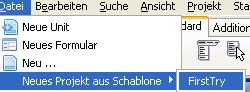
\includegraphics[width=0.3\textwidth]{Kapitel/ide/pics/PrjTempl01}}\label{fig:ProjectTempl01}Nach der Erstellung ist das Menü "`Werkzeuge"' um den Eintrag "`Optionen für Projektschablonen"' erweitert. Mit Hilfe dieses Menüpunktes kann man das Basis Verzeichnis für die Schablonen einstellen. \parpic[sr][l]{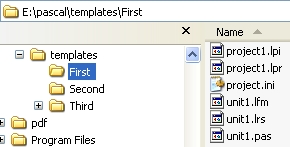
\includegraphics[width=0.3\textwidth]{Kapitel/ide/pics/PrjTempl02}}\label{fig:ProjectTempl02}Die Schablonen selbst befinden sich dann in den Unterverzeichnissen. Weiters wird auch das Menü "`Datei"' um den Eintrag "`Neues Projekt aus Schablone"' erweitert. Zusätzlich ist auch der "`Datei Neu .."' Dialog entsprechend erweitert.

Jede Schablone liegt in einem eigenen Unterverzeichnis und kann selbst weitere Unterverzeichnisse enthalten. Diese Struktur wird beim Erstellen eines neuen Projektes mittels Schablonen übertragen\footnote{Es mir in der derzeitigen Version Lazarus 0.9.25 svn 13811 nicht geglückt das die Unterverzeichnisse kopiert werden}.

Die Steuerung der Vorlagen erfolgt durch die Datei "`project.ini"'. Diese Datei ist im "`ini"' Format aufgebaut und es befinden sich derzeit zwei Sektionen darinnen. In der ersten Sektion mit dem Namen "`[Variables]"' befinden sich die Variablen\footnote{Platzhalter, veränderbare Teile}. Als Voreinstellung selbst gibt es zwei vordefinierte Variablen die die Ersetzungsroutine selbst kennt und die nicht definiert werden müssen.
\begin{description}
	\item[ProjDir]Das Verzeichnis, in welches das neue Projekt erzeugt wird
	\item[ProjName]Der Name des neuen Projektes
\end{description}
\parpic[sl][r]{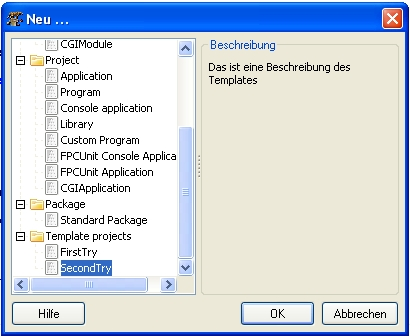
\includegraphics[width=0.4\textwidth]{Kapitel/ide/pics/PrjTempl04}}\label{fig:ProjectTempl04}Weitere Variablen, müssen in der Sektion "`[Variables]"' in der folgenden Form definiert werden. Zuerst kommt der Variablenname, dann das Gleichheitszeichen und zum Schluß eine Beschreibung, welcher in der Eingabemaske auf scheinen wird.
Während des kopierens können Ersetzungen durchgeführt werden. Das Kennzeichen für diese Ersetzung ist \_\_VARNAME\_\_\footnote{Wurde gegenüber der Beschreibung im README.txt offenbar geändert - war \$(VARNAME)}. Diese Zeichnenfolge wird durch den Inhalt der Variablen ersetzt. Die Bezeichnung "`VARNAME"' ist durch den Namen der Variable zu ersetzen. Die Ersetzung wird beim Kopieren in das neue Projekt sowohl in den Dateinamen gemacht, als auch innerhalb der Dateien. 

Die zweite Sektion beschäftigt sich mit dem beschreiben des Projektes selbst. Die Sektion "`[Project]"' beinhaltet folgende Informationen zum Projekt, wobei der Namen, Author und die Beschreibung in Datei-Neu Dialog von Lazarus angezeigt wird.
\begin{description}
	\item[Name]Namen der Vorlage
	\item[Author]Author der Vorlage
	\item[Description]Kurze Beschreibung der Vorlage, maximal einzeilig
	\item[Recurse] Ob in Unterverzeichnis hineinrekusiert\footnote{funktioniert ?!} werden soll (0=Nein, 1=Ja)
	\item[Exclude]Durch Komma getrennte Liste, welche Dateien nicht für die Ersetzung verwendet werden sollen
\end{description}	
Ist in dem Verzeichnis eine Datei mit dem Namen "`description.txt"', so wird der Inhalt der Datei als Beschreibung verwendet.

\subsubsection{Beispiel}
Als Beispiel habe ich ein vorhandenes einfaches Projekt im Vorlagen Verzeichnis abgespeichert. Weiter kommt in diese Verzeichnis eine "`project.ini"' Datei mit folgen Inhalt hinein
\begin{verbatim}
[Variables]
VarName1= Dateiname fuer das Hauptformular
[Project]
Name=SecondTry
Author= Nobody
Description= Test template 1
Recurse= 0
Exclude=
\end{verbatim}
\parpic[sr][l]{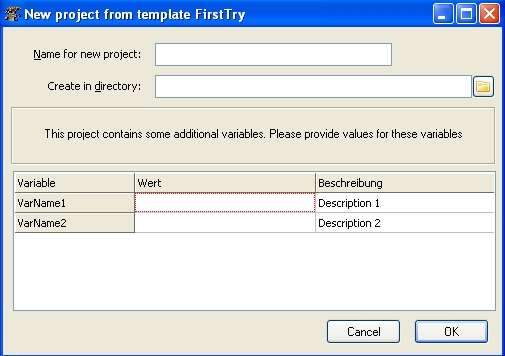
\includegraphics[width=0.3\textwidth]{Kapitel/ide/pics/PrjTempl05}}\label{fig:ProjectTempl05}
In der ersten Eingabezeile wird der Dateiname des Projektes eingegeben, er ist in der nicht sichtbaren Variablen "`ProjName"' dann vorhanden. In der zweiten Zeile gibt man den Pfad, wohin die Dateien aus den Vorlagen kopiert werden sollen an. Das kann entweder durch Direkteingabe erfolgen oder über den Dateidialog, den man rechts neben der Eingabezeile aufrufen kann. Darunter befindet sich dann die Eigabemaske für die frei (in der "`project.ini"') definierbaren Variablen. Der ausgefüllte Inhalt der Variablen ersetzt dann beim kopieren die Platzhalter.

Heisst also eine Datei im Templateverzeichnis zum Beispiel \textit{\_\_VarName1\_\_.pas} und bei der Variablen wird "`myform"' festgelegt, so wird die Datei als \textit{myform.pas} in das Zielverzeichnis kopiert. Ebenso verhält es sich mit Variablen (nicht verwechseln mit Variablen innerhalb von Lazarus), die beim kopieren ebenso durch die Werte ersetzt werden. 

Wird der Dialog jetzt bestätigt, so wird die Kopieraktion durchgeführt und Lazarus öffnet das neue Projekt.

\verb|Version: $ $ |\footnote{ Autor: Andreas Frieß\\Lizenz: GFDL}
\newpage

%###########################################################
% Code, Wie mache ich (ohne Beispiele)
%###########################################################
\chapter{Codebeispiele \& FAQ}
%--------------------------------------------------
% Sektion 
%--------------------------------------------------
\section[FAQ]{FAQ}
%%####################################################################
%    Copyright @ 2007,2008 Andreas Frieß (Friess)
%    Permission is granted to copy, distribute and/or modify this document
%    under the terms of the GNU Free Documentation License, Version 1.2
%    or any later version published by the Free Software Foundation;
%    with no Invariant Sections, no Front-Cover Texts, and no Back-Cover Texts.
%    A copy of the license is included in the section entitled ``GNU
%    Free Documentation License''.
%%####################################################################
% Created: 02.01.2008
% @cvs($Date:  $)
% @cvs($Rev: $)
% @cvs($Author: af0815 $)
% @cvs($URL: $)
%%####################################################################
\subsection{Pascal}
\subsubsection{Mit Typen arbeiten}\footnote{Aus dem Thread \textsl{http://www.lazarusforum.de/viewtopic.php?f=55\&t=4354}}
Im folgenden Beispiel wird durch die einzelnen Werte gegangen. Bei der \textit{for-Schleife} werden dabei die richtigen Grenzen beachtet. Durch die Benutzung der Bibliothek \textit{Typeinfo} ist der Zugriff auf die gespeicherten TypenInformationen möglich.
\begin{verbatim}
Uses Typinfo;

Type TSpielfarben = (rot, gruen, blau, gelb);


procedure TForm1.Button1Click(Sender: TObject);
var x  : TSpielfarben;
      s : string;
begin
  memo1.clear;
  for x := low(x) to high(x) do
  begin
    s := GetEnumName(typeinfo(TSpielfarben),ord(x));
    Memo1.Append(s);
  end;
end;

\end{verbatim}



\verb|Version: $LastChangedRevision: 59 $ |\footnote{ Autor: Andreas Frieß\\Lizenz: GFDL}
\newpage
%###########################################################
% Bibliotheken
%###########################################################
\chapter[Bibliotheken]{Bibliotheken}
%%####################################################################
%    Copyright @ 2007 Andreas Frie� (Friess)
%    Permission is granted to copy, distribute and/or modify this document
%    under the terms of the GNU Free Documentation License, Version 1.2
%    or any later version published by the Free Software Foundation;
%    with no Invariant Sections, no Front-Cover Texts, and no Back-Cover Texts.
%    A copy of the license is included in the section entitled ``GNU
%    Free Documentation License''.
%%####################################################################
% Created: 26.10.2007
% @cvs($Date: $)
% @cvs($Rev:  $)
% @cvs($Author: af0815 $)
% @cvs($URL: $)
%%####################################################################
\section[SQLdb - Serverdatenbank Komponenten]{SQLdb}
%%####################################################################
\subsection{Beschreibung}
\subsubsection{Einleitung}
SQLdb\label{SQLdb} wird speziell f�r Serverbasierende Datenbanken verwendet und besteht im Wesentlichen aus Komponenten f�r die Verbindung (TxxxConnection), f�r das Verwalten von Transaktionen (TSQLTransaction) und dem Verwalten von Datenmengen (TSQLQuery). F�r Clientdatenbanken (Dbase, FoxPro,...) sind die Komponenten unter 'Client Access'\footnote{Siehe Kapitel \ref{ClientAccess} auf Seite \pageref{ClientAccess}} vorgesehen. \parpic[sr][l]{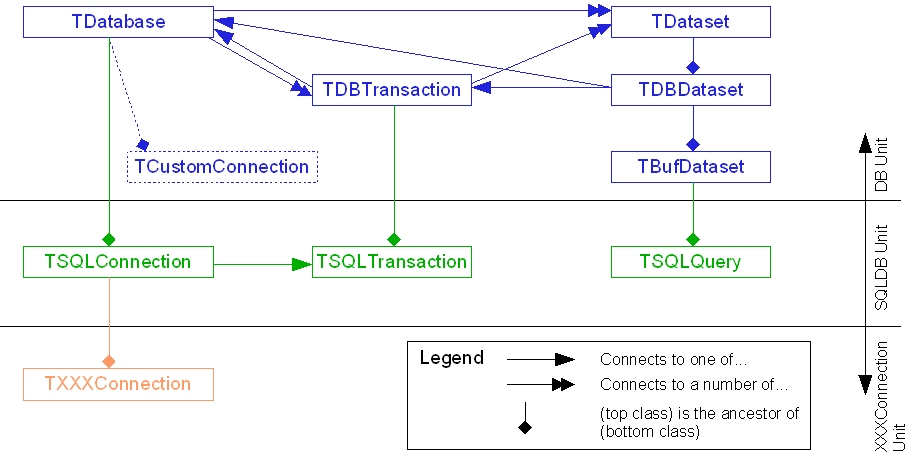
\includegraphics[width=0.5\textwidth]{Kapitel/datenbanken/pics/Laz_SqlDB_components}}
\label{fig:LazSqlDB01}
Besonders die TSQLQuery ist eine m�chtige Komponente, die einige automatismen eingebaut hat, die zwar das Leben erleichtern sollen, aber oft das Gegenteil bewirken k�nnen. In diesem Kapitel wollen wir uns die Komponenten einmal genauer ansehen. Das Bild aus der Wiki aus dem englischen Lazarusforum\cite{laz.en}\footnote{\textsl{http://wiki.lazarus.freepascal.org/SQLdb\_Programming\_Reference}} erkl�rt sch�n, wie die Komponenten zusammenh�ngen und in welchen Units sie sich befinden.

\subsubsection{Debbuging von SQLdb}
SQLdb ist ein Teil der FCL und nicht direkt von Lazarus. Die FCL wird standardm�ssig nicht mit den f�r den Debugger notwendigen Informationen kompiliert, da der Kode so kompakter und kleiner ist. Wenn man f�r die Fehlersuche es anders ben�tigt, so mu� man die fcl-db neu kompileren. Dazu mu� man die kompletten FCL Sourcen haben, dann kann man in das Verzeichnis 'fpc/packages/fcl-db' gehen und mit 'make clean all OPT='-gl'' das Paket neu kompiliren, anschliessen die neuen PPU's �ber die alten kopieren. Die Fehlersuche wird aber nur Personen empfohlen, die entsprechendes Wissen �ber die SQLdb Komponenten haben.

\subsubsection{Active, Open oder ExecSQL}
... das ist hier die Frage ? Um diese Frage zu beantworten, mu� man sich vor Augen halten, was man von der Komponente will. Mittels dem Befehl Open fordert man eine Datenmenge, die Kardinalit�t\footnote{siehe Kapitel \ref{Kardinalitaet} auf Seite \pageref{Kardinalitaet}} einer Datenmenge\footnote{siehe Kapitel \ref{Datenmenge} auf Seite \pageref{Datenmenge}} kann auch Null sein, an. Mit ExecSQL wird nur eine Aktion angefordert ohne das eine Datenmenge zur�ck erwartet wird. 
Somit ist klar, das bei allen Daten liefernden Statements das Open zu verwenden ist. Welche Statements in SQL liefern �berhaupt Datenmengen zur�ck ? Eigentlich gilt das nur f�r das 'SELECT' Statement, alle anderen ('INSERT', 'UPDATE', 'DELETE', ...) f�hren etwas aus, liefern aber keine Daten zur�ck. Ob man jetzt 'Open' verwendet oder 'Active:=true;' macht ist letztlich egal, 'Open' f�hrt genau dieses Statement aus.  

Eine Besonderheit ist die Behandlung von 'Stored Procedure' und 'Functions' auf SQL-Servern. Diese k�nnen eine Kombination im Verhalten darstellen. Dort ist dann ein ExecSQL angebracht und es k�nnen Datenmengen zur�ckgeliefert werden.

Zusammenfassung:
\begin{itemize}
	\item Open, Active: Bei der Verwendung von 'SELECT'
	\item ExecSQL: F�r alle anderen Statements 
\end{itemize}

\subsubsection{Wie kommen die ge�nderten Daten in die Datenbank}
Eine �nderung der Datenmenge alleine ist nicht ausreichend, um diese �nderung auch in der Datenbank sichtbar zu machen. Prinzipiell mu� man jetzt zwei Wege unterscheiden. Einerseits kann man �nderungen im Zuge einer Transaktion in der Datenbank festschreiben durch das Abschliessen der Transaktion oder auch durch das dezitierte schreiben durch ApplyUpdates. Ich bin der Meinung, das man sich f�r einen der Wege entscheiden sollte, wenn man eine Datenmenge �ffnet beziehungsweise anfordert. 
Arbeitet man mit Transdaktionen, dann soltte man ohne zwingenden Grund nicht mit ApplyUpdates das Transaktions\-managment st�ren.
Anderseits wenn man ohne explzite Transaktionen arbeitet, also Datenmengen �ffnet ohne vorher Transaktionen ge�ffnet zu haben, dann darf man nicht vergessen die �nderungen entweder mittels ApplyUpdates zu �bernehmen oder mittels CancelUpdates zu verwerfen. Vergisst man auf ApplyUpdates so ist dieses schlimmer als auf CancelUpdates zu vergessen. Denn ohne dem ApplyUpdates sind die Daten bei den meisten Datenbanken ganz einfach nicht in die Datenbank eingearbeitet und somit verloren.

\subsubsection{Filtern, aber wo ?}
Die Standardantwort ist im Stile von Radio Eriwan: 'Dort wo es sinnvoll ist'. Dazu mu� man sich vor Augen halten, wo man eine Datenmenge �berhaupt filtern kann. Dazu mu� man unterscheiden in Desktop Datenbanken und Server Datenbanken. 
Bei Desktop Datenbanken kann die Frage schon obsolet sein, weil die Datenmenge sowieso nur lokal gefiltert werden kann. 
Bei Datenbankenservern schaut die Sachlage ganz anders aus. Denn die k�nnen Datenmengen sehr wohl, effizient vor verarbeiten und nur die wenigen Ergebnisse zur�ck transportieren. Damit wird am lokalen Rechner Netzwerkleistung, Speicher und Resourcen geschont. Somit kann man hier dem filtern am Server den Vorzug geben. Werden aber Daten erst am lokalen Rechner verkn�pft, so kann man oft nur lokal filtern. 
Somit ist klar, das es stark auf das Design der Applikation an kommt, was sinnvoll ist.  

\subsubsection{Anzahl der Datens�tze abfragen}
Hier kann man generell zwei verschiedene F�lle unterscheiden. Einmal den Fall, das man wissen will, ob �berhaupt Datens�tze vorhanden sind und dem Fall, das man die Anzahl wissen will. 

Generell ist es nur dann sinnvoll die Anzahl der Datens�tze zu bestimmen, wenn eine Abfrage aktiv ist.

Ob Datens�tze �berhaupt vorhanden sind, kann man �ber die Abfrage von EOF\footnote{End of File - Anfang der Daten} und BOF\footnote{Beginn of File - Ende der Daten} machen. Sind beide vorhanden ('true') so mu� die Datenmenge leer sein. Genau diese macht die Methode 'IsEmpty'. Somit kann man diese genau f�r diesen Fall verwenden.

Die Anzahl selbst der Datens�tze, kann man theoretisch mittels der Eigenschaft 'RecordCount' abfragen. Alledings mu� dazu auch der Datenbanktreiber\footnote{Ist genaugenommen die Verbindungskomponente} das unterst�tzen. Bis jetzt ist die Unterst�tzung auch nicht wirklich vorhanden. Weiters handelt es sich hier eher um eine Eigenschaft von Desktopdatenbanken, denn dort kann die Anzahl der Datens�tze nicht anders festgestellt werden.

Die andere Variante die sich daher anbietet ist die SQL Abfrage selbst. So kann man mittels dem SQL-Statement \verb|select count(row1) as Anzahl from table1 where ...| die Anzahl ermitteln.

%
%Methoden .RecordCount:
%Ein 'select count(row1) as Anzahl from table1 where ... ' bringt die Information auch (Server). Warum jetzt RecordCount nicht funktioniert m�sst ich mir ansehen. Du hast es aber auf eine vorhandene ge�ffnete Datenmenge anzuwenden probiert ?

\subsubsection{Navigieren durch eine Datenmenge}
F�r das Navigieren durch die Datenmenge stehen ein paar Befehle zur Verf�gung. Mit 'first' kommt man zum ersten, mit 'last' zum letzten, mit 'next' springt man auf den n�chsten und mit mit 'prior' zum vorhergehenden Datensatz. Gr��ere Bewegungen kann man mit 'MoveBy' machen. Das funktioniert vorw�rts mit positiven Zahlen, r�ckw�rts mit negativen Zahlen. Allerdings mu� man bedenken, das ein 'MoveBy' nicht zwingend die volle Distanz verfahren kann, wenn die Grenzen der Datenmenge erreicht werden. Wenn also ein EOF oder BOF nach dem 'MoveBy' ansteht, so wird nicht die volle Distanz erreicht worden sein, man wei� aber nicht um wie viel verfahren wurde.

\subsubsection{Was ist BOF und EOF}
'BOF' bedeutet das man in der Datenmenge am Anfang, bei 'EOF'  am Ende der Datenmenge steht. Wenn zum gleichen Zeitpunkt beide vorhanden sind, so ist das ein Zeichen, das die Datenmenge null ist.

\subsubsection{Zugriff auf Felder}
Auf die Felder\footnote{auch Attribute genannt} kann �ber die Eigenschaft 'Fields' zugegriffen werden. Zus�tzlich kann �ber die Methode 'FieldByName' mittels des Feldnamens oder 'FieldByNumber' einfach auf die einzelnen Felder zugegriffen werden. Die Werte werden �ber die 'Values' Eigenschaft als variant zugewiesen oder �ber die entsprechenden 'AsInteger', 'AsString' und 'As.....'. 

\subsubsection{Zugriff auf Parameter}
Auf die Felder der Parameter kann �ber die Eigenschaft 'Params' zugegriffen werden.Zus�tzlich kann �ber die Methode 'ParamsByName' mittels des Feldnamens einfach auf die einzelnen Felder zugegriffen werden. Die Werte werden �ber die 'Values' Eigenschaft als variant zugewiesen oder �ber die entsprechenden 'AsInteger', 'AsString' und 'As.....'. 

Im SQL-Statement werden die Parameter durch einen Doppelpunkt am Anfang des Names kenntlich gemacht. Zum Beispiel: \verb|insert tablex (row1, row2) values (:param1, :param2)| Hier ist ':param1' einer der Parameter. Die Zuweisung im Programm erfolgt �ber \verb|TQ1.Params.ParamByName('param1').value := 'test';|.

\subsubsection{Schl�sselfelder}
Als Schl�sselfelder werden die Felder\footnote{Schl�ssel k�nnen �ber mehrere Felder gehen um eindeutig zu sein, oder weil sie zusammengesetzt sind} bezeichnet in dem der prim�re Schl�ssel der Tabelle gespeichert ist. Dieser sollte bei jeder �nderbaren Datenmenge definiert sein, damit die Komponenente richtig die Datens�tze �ndern oder l�schen kann. Schl�ssel erzwingen eine Eindeutigkeit.

% Auf usePrimaryKeyAsKey nicht vergessen.

%%####################################################################
\subsection{TxxxConnection}
Genau genommen handelt es sich hier nicht nur um eine einfache Deklaration der Verbindung sondern um den lokalen Verwaltungsteil der Datenbank. 
Hier werden die gemeinsamen Methoden und EIgenschaften behandelt, im Folgenden die verschiedenen Connection mit den abweichenden Details behandelt.

\subsubsection{Close}
\begin{description}
  \item \texttt{procedure Close;}\\Setzt ganz einfach die E�genschaft active auf false.
  \begin{description}
    \item Methode von TxxxConnection>TSQLConnection>TDatabase>TCustomConnection
  \end{description}
\end{description}

\subsubsection{EndTransaction}
\begin{description}
  \item \texttt{procedure EndTransaction; override;}\\Ruft die entsprechede Methode der Komponente Transaction auf.
  \begin{description}
    \item Methode von TxxxConnection>TSQLConnection
  \end{description}
\end{description}

\subsubsection{ExecuteDirect}
\begin{description}
  \item \texttt{procedure ExecuteDirect(SQL : String); overload; virtual;}
  \item \texttt{procedure ExecuteDirect(SQL : String; ATransaction : TSQLTransaction); overload; virtual;}\\F�hrt das SQL-Statement entweder im Kontext der default Transaktion oder mittels der Angegeben Transaktion aus.
  \begin{description}
    \item Methode von TxxxConnection>TSQLConnection
  \end{description}
  \begin{description}
    \item Parameter
    \begin{description}
      \item[SQL: string] Das auszuf�hrende SQL-Statement
      \item[ATransaction : TSQLTransaction] Die Transaktion in deren Kontext das SQL-Statement durchgef�hrt wird. 
    \end{description}
  \end{description}
\end{description}

\subsubsection{GetFieldNames}
\begin{description}
  \item \texttt{procedure GetFieldNames(const TableName : string; List :  TStrings); virtual;}\\Ermittelt die Namen der Felder der Tabelle.
  \begin{description}
    \item Methode von TxxxConnection>TSQLConnection
  \end{description}
  \begin{description}
    \item Parameter
    \begin{description}
      \item[TableName : string;] Name der Tabelle deren Felder ermittelt werden sollen
      \item[List : TStrings;] Die Liste der Felder
    \end{description}
  \end{description}
\end{description}

\subsubsection{GetProcedureNames}
\begin{description}
  \item \texttt{procedure GetProcedureNames(List : TStrings); virtual;}\\Ermittelt die Namen der gespeicherten Prozeduren.
  \begin{description}
    \item Methode von TxxxConnection>TSQLConnection
  \end{description}
  \begin{description}
    \item Parameter
    \begin{description}
      \item[List : TStrings;] Die Liste der Prozeduren
    \end{description}
  \end{description}
\end{description}

\subsubsection{GetTableNames}
\begin{description}
  \item \texttt{procedure GetTableNames(List : TStrings; SystemTables : Boolean = false); virtual;}\\Ermittelt die Tabellennamen oder die Systemtabellennamen (abh�ngig von SystemTables)
  \begin{description}
    \item Methode von TxxxConnection>TSQLConnection
  \end{description}
  \begin{description}
    \item Parameter
    \begin{description}
      \item[List : TStrings;] Die Liste der Tabellennamen
      \item[SystemTables : Boolean] Ob Systentabellen (true) oder Usertabellen (false) ermittelt werden sollen.
    \end{description}
  \end{description}
\end{description}

\subsubsection{Open}
\begin{description}
  \item \texttt{procedure Open;}\\Setzt ganz einfach die E�genschaft active auf true.
  \begin{description}
    \item Methode von TxxxConnection>TSQLConnection>TDatabase>TCustomConnection
  \end{description}
\end{description}

\subsubsection{StartTransaction}
\begin{description}
  \item \texttt{procedure StartTransaction; override;}\\Ruft die entsprechede Methode der Komponente Transaction auf.
  \begin{description}
    \item Methode von TxxxConnection>TSQLConnection
  \end{description}
\end{description}

\subsubsection{CharSet}
\begin{description}
  \item \texttt{property CharSet : string read FCharSet write FCharSet;}\\
  \begin{description}
    \item Eigenschaft von TxxxConnection>TSQLConnection
  \end{description}
  \begin{description}
    \item Zugriff: Lesend und schreibend
  \end{description}
\end{description}

\subsubsection{Connected}
\begin{description}
  \item \texttt{property Connected: Boolean read FConnected write SetConnected;}\\Gibt an ob die Verbindung besteht oder nicht. True aktiviert die Verbindung.
  \begin{description}
    \item Eigenschaft von TxxxConnection>TSQLConnection>TDatabase
  \end{description}
  \begin{description}
    \item Zugriff: Lesend und schreibend
  \end{description}
\end{description}

\subsubsection{DatabaseName}
\begin{description}
  \item \texttt{property DatabaseName: string read FDatabaseName write FDatabaseName;}\\Gibt den Namen der Datenbank an. Ist f�r die verschiedenen Datenbanken unterschiedlich. Siehe bei den entsprechenden Verbindungen.
  \begin{description}
    \item Eigenschaft von TxxxConnection>TSQLConnection>TDatabase
  \end{description}
  \begin{description}
    \item Zugriff: Lesend und schreibend
  \end{description}
\end{description}

\subsubsection{HostName}
\begin{description}
  \item \texttt{property HostName : string Read FHostName Write FHostName;}\\Gibt den Namen des Hosts (Server) an auf welchen sich die Datenbank befindet. Bei lokalen Server ist das 'localhost' oder auch '127.0.0.1'.
  \begin{description}
    \item Eigenschaft von TxxxConnection>TSQLConnection
  \end{description}
  \begin{description}
    \item Zugriff: Lesend und schreibend
  \end{description}
\end{description}

\subsubsection{KeepConnection}
\begin{description}
  \item \texttt{property KeepConnection;}\\ToDo
  \begin{description}
    \item Eigenschaft von TxxxConnection>TSQLConnection>TDatabase
  \end{description}
  \begin{description}
    \item Zugriff: Lesend und schreibend
  \end{description}
\end{description}

\subsubsection{LoginPrompt}
\begin{description}
  \item \texttt{property LoginPrompt: Boolean read FLoginPrompt write FLoginPrompt;}\\Gibt an ob ein Login Prompt beim verbinden automatisch erzeugt werden soll.
  \begin{description}
    \item Eigenschaft von TxxxConnection>TSQLConnection>TDatabase>TCustomConnect
  \end{description}
  \begin{description}
    \item Zugriff: Lesend und schreibend
  \end{description}
\end{description}

\subsubsection{Params}
\begin{description}
  \item \texttt{property Params : TStrings read FParams Write FParams;}\\Enth�lt spezielle Parameter f�r die Verbindung.
  \begin{description}
    \item Eigenschaft von TxxxConnection>TSQLConnection>TDatabase
  \end{description}
  \begin{description}
    \item Zugriff: Lesend und schreibend
  \end{description}
\end{description}

\subsubsection{Password}
\begin{description}
  \item \texttt{}\\Enth�lt das Passwort f�r die Verbindung. Nicht ben�tigt, wenn LoginPrompt true ist.
  \begin{description}
    \item Eigenschaft von TxxxConnection>TSQLConnection>TDatabase
  \end{description}
  \begin{description}
    \item Zugriff: Lesend und schreibend
  \end{description}
\end{description}

\subsubsection{Role}
\begin{description}
  \item \texttt{Property Role :  String read FRole write FRole;}\\ToDo
  \begin{description}
    \item Eigenschaft von TxxxConnection>TSQLConnection
  \end{description}
  \begin{description}
    \item Zugriff: Lesend und schreibend
  \end{description}
\end{description}

\subsubsection{StreamedConnected}
\begin{description}
  \item \texttt{property Streamedconnected: Boolean read FStreamedConnected write FStreamedConnected;}\\ToDo
  \begin{description}
    \item Eigenschaft von TxxxConnection>TSQLConnection>TDatabase>TCustomConnection
  \end{description}
  \begin{description}
    \item Zugriff: Lesend und schreibend
  \end{description}
\end{description}

\subsubsection{Transaction}
\begin{description}
  \item \texttt{property Transaction : TSQLTransaction read FTransaction write SetTransaction;}\\Gibt die Transaktions Komponente an.
  \begin{description}
    \item Eigenschaft von TxxxConnection>TSQLConnection
  \end{description}
  \begin{description}
    \item Zugriff: Lesend und schreibend
  \end{description}
\end{description}

\subsubsection{UserName}
\begin{description}
  \item \texttt{property UserName : string read FUserName write FUserName;}\\Enth�lt den Benutzernamen f�r die Verbindung beziehungsweise f�r den Zugriff auf die Datenbank.
  \begin{description}
    \item Eigenschaft von TxxxConnection>TSQLConnection
  \end{description}
  \begin{description}
    \item Zugriff: Lesend und schreibend
  \end{description}
\end{description}

Jede Datenbank hat ihre spezielle Verbindung (Connection).

%  Public
%    Property ServerInfo : String Read FServerInfo;
%    Property HostInfo : String Read FHostInfo;
%    property ClientInfo: string read GetClientInfo;
%    property ServerStatus : String read GetServerStatus;
%  published
%    property Dialect  : integer read FDialect write FDialect;
%  end;
\subsection{TMySQL50Connection}
Jede Datenbank hat ihre spezielle Verbindung (Connection). Dies hier ist die Verbindung zu MySQL 5.0

\subsection{TMySQL41Connection}
Jede Datenbank hat ihre spezielle Verbindung (Connection). Dies hier ist die Verbindung zu MySQL 4.1

\subsection{TMySQL40Connection}
Jede Datenbank hat ihre spezielle Verbindung (Connection). Dies hier ist die Verbindung zu MySQL 4.0

\subsection{TOracleConnection}
Jede Datenbank hat ihre spezielle Verbindung (Connection). Dies hier ist die Verbindung zu Oracle.

\subsection{TPQConnection}
Jede Datenbank hat ihre spezielle Verbindung (Connection). Dies hier ist die Verbindung zu PostGreSQL Datenbanken.

\subsection{TODBCConnection}
Jede Datenbank hat ihre spezielle Verbindung (Connection). Dies hier ist die Verbindung zu den ODBC Treibern.

%%####################################################################
\subsection{TSQLTransaction}
Als Transaktion wird eine feste Folge von Operationen, die eine Einheit bilden, bezeichnet. Transaktionen m�ssen die ACID-EIgenschaft garantieren. A) Atomit�t, das hei�t untrennbar. Es wird entweder alles oder nichts durchgef�hrt. C) Konsistenz, Nach der Transaktion m�ssen die Daten konsistent sein. Daher auch an allen ge�nderten Stellen den gleichen Inhalt haben. I) Isolation, mehrere gelichzeitig laufende Transaktionen d�rfen sich nicht gegenseitig beeinflussen. D) Dauerhaft, die Auswirkungen der Transaktion m�ssen im Datenbestand dauerhaft sein. Auch bei widrigen Umst�nden d�rfen die Transaktionen nicht verloren gehen oder vergessen werden, zB. bei R�cksicherungen nach Absturz.

Der Ablauf einer Transaktion ist relativ einfach. Die Transaktion wird er�ffnet, dann die Handlungen an der Datenbank gesetzt und die Transaktion entweder mit 'Rollback' wenn sie zur�ckgenommen werden soll oder mit 'Commit' wenn die �nderderungen dauerhaft �bernommen werden sollten, abgeschlossen.  

Man mu� sich nur vor Augen halten, das das Datenbanksystem um die ACID Eigenschaften garantieren zu k�nnen, Aktionen wie Sperren, Duplizieren oder auch Warten durchf�hren mu�. Deshalb soll eine Transaktion nur solange aufrecht erhalten werden wie es unbedingt n�tig ist. Das heisst, auch, w�hrend einer Benutzereingabe oder sonstiger Wartezeit sollte keine Transaktion stattfinden. Besonders bei Mehrbenutzersystemen kann das bis zum Stillstand der Datenbank f�hren, wenn wegen vergessener Eingabe bei Arbeitscschlu� eine Transaktion aktiv bleibt und deshalb eine Sperre auf einer Datenbank liegt.

\subsubsection{Commit}
\begin{description}
  \item \texttt{procedure Commit; virtual;}\\Schliesst die Transaktion ab
  \begin{description}
    \item Methode von TSQLTransaction
  \end{description}
\end{description}

\subsubsection{CommitRetaining}
\begin{description}
  \item \texttt{procedure CommitRetaining; virtual;}\\F�hrt ein Commit durch, l�sst aber die Datenmenge offen. Wenn es die Datenbank nicht unterst�tzt, so wird es von der SQLdb Komponete simmuliert.
  \begin{description}
    \item Methode von TSQLTransaction
  \end{description}
\end{description}

\subsubsection{EndTransaction}
\begin{description}
  \item \texttt{procedure EndTransaction; override;}\\Beendet die Transaktion, f�hrt ein normalerweise ein Rollback durch.
  \begin{description}
    \item Methode von TSQLTransaction
  \end{description}
\end{description}

\subsubsection{Rollback}
\begin{description}
  \item \texttt{procedure Rollback; virtual;}\\Rollt die Transaktion zur�ck, macht daher die �nderungen nicht aktiv.
  \begin{description}
    \item Methode von TSQLTransaction
  \end{description}
\end{description}

\subsubsection{RollbackRetaining}
\begin{description}
  \item \texttt{procedure RollbackRetaining; virtual;}\\F�hrt ein Rollback durch, l�sst aber die Datenmenge offen. Wenn es die Datenbank nicht unterst�tzt, so wird es von der SQLdb Komponete simmuliert.
  \begin{description}
    \item Methode von TSQLTransaction
  \end{description}
\end{description}

\subsubsection{StartTransaction}
\begin{description}
  \item \texttt{procedure StartTransaction; override;}\\Startet die Transaktion
  \begin{description}
    \item Methode von TSQLTransaction
  \end{description}
\end{description}

\subsubsection{Action}
\begin{description}
  \item \texttt{property Action : TCommitRollbackAction read FAction write FAction;}\\ToDo
  \begin{description}
    \item Eigenschaft von TSQLTransaction
  \end{description}
  \begin{description}
    \item Zugriff: Lesend und schreibend
  \end{description}
\end{description}

\subsubsection{Database}
\begin{description}
  \item \texttt{Property DataBase : TDatabase Read FDatabase Write SetDatabase;}\\Gibt den Namen der Verbindung (=Datenbank) an.
  \begin{description}
    \item Eigenschaft von TSQLTransaction>TDBTransaction
  \end{description}
  \begin{description}
    \item Zugriff: Lesend und schreibend
  \end{description}
\end{description}

\subsubsection{Params}
\begin{description}
  \item \texttt{property Params : TStrings read FParams Write FParams;}\\Enth�lt spezielle Parameter f�r die Verbindung.
  \begin{description}
    \item Eigenschaft von TxxxConnection>TSQLConnection>TDatabase
  \end{description}
  \begin{description}
    \item Zugriff: Lesend und schreibend
  \end{description}
\end{description}



%%####################################################################
\subsection{TSQLQuery}
\subsubsection{Allgemeines}
Der Name beschreibt nur unzureichend die Komponente. Es ist nicht nur ein Beh�lter f�r Abfragen (Query) sondern die Kapselung f�r die Datenmenge. Das heisst, �ber die Komponente l�uft eigenlich alles bez�glich Daten und Datenmenge. Sie wird sowohl f�r DDL\footnote{Datendefinitionssprache siehe Kapitel \ref{DDL} auf Seite \pageref{DCL}}, DML\footnote{Datenver�nderungssprache siehe Kapitel \ref{DML} auf Seite \pageref{DCL}} und DCL\footnote{Datenkontrollsprache siehe Kapitel \ref{DCL} auf Seite \pageref{DCL}} verwendet


\subsubsection{Methoden von TSQLQuery}
Im folgenden sind hier die wichtigsten Methoden beschrieben. Standardmethoden wie 'Create' oder 'Free' werden hier nicht beschrieben.

\subsubsection{ApplyUpdates}
\begin{description}
  \item \texttt{procedure ApplyUpdates; virtual; overload;}
  \item \texttt{procedure ApplyUpdates(MaxErrors: Integer); virtual; overload;}\\�bertr�gt die �nderungen von der Datenmenge in die Datenbank. 'ApplyUpdates' entspricht 'ApplyUpdates(0)'.
  \begin{description}
    \item Methode von TSQLQuery>TBufDataset
  \end{description}
\end{description}

\subsubsection{CancelUpdates}
\begin{description}
  \item \texttt{procedure CancelUpdates; virtual;}\\Die �nderungen an der Datenmenge werden verworfen.
  \begin{description}
    \item Methode von TSQLQuery>TBufDataset
  \end{description}
\end{description}

\subsubsection{Close}
\begin{description}
  \item \texttt{procedure Close;}\\
Setzt die Eigenschaft 'Active' auf 'false'. Somit wird die Datenmenge geschlossen.
  \begin{description}
    \item Methode von TSQLQuery
  \end{description}
\end{description}

\subsubsection{ExecSQL}
\begin{description}
  \item \texttt{procedure ExecSQL;}\\
F�hrt die in der Eigenschaft SQL definierten SQL-Befehle aus, liefert aber keine Datenmenge zur�ck. Sonderfall 'Stored Procedure' kann unter umst�nden Datenmengen zur�ck liefern. 
  \begin{description}
    \item Methode von TSQLQuery
  \end{description}
\end{description}

\subsubsection{IsEmpty}
\begin{description}
  \item \texttt{function IsEmpty: Boolean;}\\
�berpr�ft ob die Datenmenge leer ist. Gibt true zur�ck, wenn die Datenmenge leer ist. Zu beachten ist, das das Ergebnis immer false ist, wenn die Datenmenge im Zustand 'dsinsert' ist, sprich ein Datensatz eingef�gt wird. Ausserdem ist die Pr�fung nur dann sinnvoll wenn eine Abfrage aktiv ist.
  \begin{description}
    \item Methode von TSQLQuery>TBufDataset>TDBDataset>TDataSet
  \end{description}
\end{description}

\subsubsection{Locate}
\begin{description}
  \item \texttt{function Locate(const keyfields: string; const keyvalues: Variant; options: TLocateOptions) : boolean; override;}\\ Achtung, es ist derzeit nur m�glich in einem Feld zu suchen, nicht in mehreren. Beim Suchen selbst sind keine Wildcards erlaubt ('*', '\%',...)
  \begin{description}
    \item Methode von TSQLQuery>TBufDataset
  \end{description}
  \begin{description}
    \item Parameter
    \begin{description}
      \item[keyfields: string] Angabe des Suchfeldes
      \item[keyvalues: Variant] Inhalt nach dem gesucht wird
      \item[options: TLocateOptions] Scheibweise egal 'loCaseInsensitive', nur eine Teilmenge 'loPartialKey'
    \end{description}
  \end{description}
\end{description}

\subsubsection{Open}
\begin{description}
  \item \texttt{procedure Open;}\\
F�hrt die in der Eigenschaft SQL definierten SQL-Befehle aus und liefert die Datenmenge zur�ck. Intern wird die Eigenschaft 'Active' auf 'true' gesetzt.
  \begin{description}
    \item Methode von TSQLQuery
  \end{description}
\end{description}

\subsubsection{Prepare}
\begin{description}
  \item \texttt{procedure Prepare;}\\
Mittels Prepare wird die Komponente darauf vorbereitet, das es den Ablauf optimieren kann. Die Komponente geht davon aus, das das SQL-Statement endg�ltig ist, nur mehr die Parameter k�nnen sich �ndern. Somit k�nnen die Statement verarbeitet werden und die Verbindungen vorbereitet. Die Komponente kann die Staements an die Server leiten und diese k�nnen die Befehle jetzt vorkompilieren und optimieren.
  \begin{description}
    \item Methode von TSQLQuery
  \end{description}
\end{description}

\subsubsection{SetSchemaInfo}
\begin{description}
  \item \texttt{procedure SetSchemaInfo( SchemaType : TSchema\-Type; Schema\-Object\-Name, Schema\-Pattern : string);}\\
Setzt das Schema, die aktuellen SQL Statements gehen dabei verloren und werden durch die neuen Informationen ersetzt. Zus�tzlich wird der Datenbankzugriff auf nur lesen gesetzt.
  \begin{description}
    \item Methode von TSQLQuery
  \end{description}
  \begin{description}
    \item Parameter
    \begin{description}
      \item[SchemaType : TSchemaType] Kann folgende Werte annehmen: stNoSchema, stTables, stSysTables, stProcedures, stColumns, stProcedureParams, stIndexes, stPackages.
      \item[SchemaObjectName : string] 
      \item[SchemaPattern : string]
    \end{description}
  \end{description}
\end{description}

\subsubsection{Unprepare}
\begin{description}
  \item \texttt{procedure Unprepare;}\\
Setzt die durch Prepare ausgel�sten Vorverarbeitungen zur�ck. Sollte immer vor �nderungen an der Komponente aufgerufen werden, wenn man Prepare verwendet hat.
  \begin{description}
    \item Methode von TSQLQuery
  \end{description}
\end{description}

\subsubsection{UpdateStatus}
\begin{description}
  \item \texttt{function UpdateStatus: TUpdateStatus; override;}\\
Gibt den Status des Zwischenspeicher f�r ge�nderte Daten an. Kann folgende zust�nde annehmen : Keine �nderungen ist 'usUnmodified', bei �nderungen 'usModified', Einf�gungen 'usInserted' und bei L�schungen 'usDeleted'.
  \begin{description}
    \item Methode von TSQLQuery>TBufDataset
  \end{description}
\end{description}

%*******************
\subsubsection{Eigenschaften von TSQLQuery}
Hier beginnt die Beschreibung der wichtigsten Eigenschaften und Ereignisse. Wie schon bei den Methoden, werden hier nur die wichtigsten erl�utert. 

\subsubsection{Active}
\begin{description}
  \item \texttt{property Active: Boolean read GetActive write SetActive default False;}\\ Sagt aus ob die Komponente derzeit aktiv ist und eine Datenmenge zur�ckliefert. Ein setzen auf 'true' entspricht der Methode 'Open' und ein setzen auf 'false' entspricht der Methode 'Close'.
  \begin{description}
    \item Eigenschaft von TSQLQuery
  \end{description}
  \begin{description}
    \item Zugriff: Lesend und schreibend
    \item Defaultwert: false
  \end{description}
\end{description}

\subsubsection{Database}
\begin{description}
  \item \texttt{property Database;}\\Gibt die zust�ndige Databasekomponente (TxxxConnection) an.
  \begin{description}
    \item Eigenschaft von TSQLQuery
  \end{description}
  \begin{description}
    \item Zugriff: Lesend und schreibend
  \end{description}
\end{description}

\subsubsection{DataSource}
\begin{description}
  \item \texttt{Property DataSource : TDatasource;}\\WIrd in einer Master-Detail Beziehung vom der Client-Query zur Synchronisierung mit der Master-Query verwendet verwendet.
  \begin{description}
    \item Eigenschaft von TSQLQuery
  \end{description}
  \begin{description}
    \item Zugriff: Lesend und schreibend
    \item Defaultwert: false
  \end{description}
\end{description}

\subsubsection{Filter}
\begin{description}
  \item \texttt{property Filter: string read FFilterText write SetFilterText;}\\Enth�lt den Filter f�r die Datenmenge, wenn definiert. Entspricht einer 'WHERE'-Klausel bei einem SQL Statement - siehe auch 'Serverfiltered'. Normalerweise ist eine Filterung am Server vorzuziehen, da die transportierte Datenmenge geringer ist. 
Wird erst aktiv durch aktivieren der Eigenschaft 'Filtered'.
  \begin{description}
    \item Eigenschaft von TSQLQuery
  \end{description}
  \begin{description}
    \item Zugriff: Lesend und schreibend
  \end{description}
\end{description}

\subsubsection{Filtered}
\begin{description}
  \item \texttt{property Filtered: Boolean read FFiltered write SetFiltered default False;}\\Gibt an ob die Datenmenge gefiltert ist. Ein setzen der Eigenschaft bewirkt, das der Filter aktiv wird und die Datenmenge entsprechend eingeschr�nkt wird. 
  \begin{description}
    \item Eigenschaft von TSQLQuery
  \end{description}
  \begin{description}
    \item Zugriff: Lesend und schreibend
  \end{description}
\end{description}

\subsubsection{FilterOptions}
\begin{description}
  \item \texttt{property FilterOptions: TFilterOptions read FFilterOptions write SetFilterOptions;}\\M�glich sind 'foCaseInsensitive' ignoriert Gro�-, Kleinschreibung und 'foNoPartialCompare' schaltet die Erkennung von Teilen beim Filtern aus. Wirkt nur auf die lokale Filterung und nicht auf die Serverfilter.
  \begin{description}
    \item Eigenschaft von TSQLQuery>TBufDataset>TDBDataset>TDataSet
  \end{description}
  \begin{description}
    \item Zugriff: Lesend und schreibend
  \end{description}
\end{description}

\subsubsection{Params}
\begin{description}
  \item \texttt{property Params : TParams;}\\Enth�lt die Parameter f�r die SQLStatements
  \begin{description}
    \item Eigenschaft von TSQLQuery
  \end{description}
  \begin{description}
    \item Zugriff: Lesend und schreibend
  \end{description}
\end{description}

\subsubsection{ParseSQL}\label{ParseSQL}
\begin{description}
  \item \texttt{property ParseSQL : Boolean;}\\Mit dieser Eigenschaft wird angezeigt ob die Komponente den SQL-Text auswerten soll. Soll sie den SQL-Text auswerten, so kann der Text f�r die Optimierung der Indexe etwas umgestellt werden. Weiters wird dann auch UsePrimaryKeyAsKey ausgewertet und zus�tzlich, wenn nicht schon vorhanden, die Vorbereitungen f�r die UpdateSQl, DeleteSQL und InsertSQL durchgef�hrt. Es kann sein, das die Query in machen f�llen schlecht ausgewertet wird, was sich durch dubiose SQLFehler zeigt. Dann kan man versuchen das ParseSQL und UsePrimaryKeyAsKey auszuschalten und alle Queries von Hand richtig zu setzen.   
  \begin{description}
    \item Eigenschaft von TSQLQuery
  \end{description}
  \begin{description}
    \item Zugriff: Lesend und schreibend
  \end{description}
\end{description}

\subsubsection{Prepared}
\begin{description}
  \item \texttt{property Prepared : boolean read IsPrepared;}\\Gibt den Status an, ob die Komponente Vorverarbeitung aktiviert hat.
  \begin{description}
    \item Eigenschaft von TSQLQuery
  \end{description}
  \begin{description}
    \item Zugriff: Nur lesend
  \end{description}
\end{description}

\subsubsection{ReadOnly}
\begin{description}
  \item \texttt{property ReadOnly : Boolean;}\\Zeigt an ob auf die Datenmenge nur lesend zugegriffen werden kann.
  \begin{description}
    \item Eigenschaft von TSQLQuery
  \end{description}
  \begin{description}
    \item Zugriff: Nur lesend
  \end{description}
\end{description}

\subsubsection{RecordCount}
\begin{description}
  \item \texttt{property RecordCount: Longint read GetRecordCount;}\\Ob die Eigenschaft verf�gbar ist, h�ngt von der Connectionkomponente ab. Wenn nichts implementiert wird, so kommt bei einer Abfrage der Wert '-1' zur�ck. Ansonsten die Anzahl der Datens�tze der Abfrage. Sinnvoller weise sollte eine Abfrage aktiv sein, ansonsten kann es zu Laufzeitfehlern kommen.
  \begin{description}
    \item Eigenschaft von TSQLQuery>TBufDataset>TDBDataset>TDataSet
  \end{description}
  \begin{description}
    \item Zugriff: Nur lesend
  \end{description}
\end{description}

\subsubsection{ServerFilter}
\begin{description}
  \item \texttt{property ServerFilter: string read FServer\-Filter\-Text write Set\-Server\-Filter\-Text;}\\Enth�lt den Filter f�r die Datenmenge, wenn definiert. Intern wird der Filter in eine 'WHERE'-Klausel umgesetzt. Somit erfolgt die Filterung bereits am Server. Wird erst aktiv durch aktivieren der Eigenschaft 'ServerFiltered'.
  \begin{description}
    \item Eigenschaft von TSQLQuery
  \end{description}
  \begin{description}
    \item Zugriff: Nur Lesend
  \end{description}
\end{description}

\subsubsection{ServerFiltered}
\begin{description}
  \item \texttt{property ServerFiltered: Boolean read FServer\-Filtered write Set\-Server\-Filtered default False;}\\Gibt an ob die Datenmenge am Server gefiltert ist. Ein setzen der Eigenschaft bewirkt, das der Filter am Server aktiv wird und die Datenmenge dort entsprechend eingeschr�nkt wird. 
  \begin{description}
    \item Eigenschaft von TSQLQuery
  \end{description}
  \begin{description}
    \item Zugriff: Lesend und schreibend
  \end{description}
\end{description}

\subsubsection{SQL, UpdateSQL, InsertSQL, DeleteSQL}
\begin{description}
  \item \texttt{property SQL : TStringlist;}
  \item \texttt{property UpdateSQL : TStringlist;}
  \item \texttt{property InsertSQL : TStringlist;}
  \item \texttt{property DeleteSQL : TStringlist;}\\In SQL befindet sich das SQL Statement was ausgef�hrt werden soll. Ist es ein einfacheres Select-Statement so kann TSQLQuery auch automatisch die Statements f�r �nderungen (UpdateSQL), Einf�gen (InsertSQL) und L�schen (DeleteSQL) ausf�llen. Ist das SQL Statement komplexer so geht diese automatik manchmal ins Leere, kann die Statements nicht richtig auswerten und verursacht unerkl�rliche Probleme.\\
UpdateSQL: Hier stehen die SQL Statements um �nderungen in der Datenmenge durchzuf�hren.\\
InsertSQL: Die Statements um Datens�tze einzuf�gen.\\
DeleteSQL: Statements um Datens�tze zu l�schen.\\
Die SQL Statements interaktieren mit der Eigenschaft ReadOnly, UsePrimaryKeyAsKey, ParseSQL, IndexDefs und Params (Vielleicht auch einigen mehr). Wenn die Komponente nicht so reagiert wie erwartet, dann sollte man sich das SQL und die vorher genannten Eigenschaften n�her ansehen.
  \begin{description}
    \item Eigenschaft von TSQLQuery
  \end{description}
  \begin{description}
    \item Zugriff: Lesend und schreibend
  \end{description}
\end{description}

\subsubsection{Transaction}
\begin{description}
  \item \texttt{property Transaction;}\\Gibt die zust�ndige Transaktionskomponente an.
  \begin{description}
    \item Eigenschaft von TSQLQuery
  \end{description}
  \begin{description}
    \item Zugriff: Lesend und schreibend
  \end{description}
\end{description}

\subsubsection{StatementType}
\begin{description}
  \item \texttt{property StatementType : TStatementType read GetStatementType;}\\M�glich sind 'stNone', 'stSelect', 'stInsert', 'stUpdate', 'stDelete', 'stDDL', 'stGetSegment', 'stPutSegment', 'stExecProcedure', 'stStartTrans', 'stCommit', 'stRollback' und 'stSelectForUpd'. Es wird hier der Komponente mitgeteilt, wie sie den Text in der Eingeschaft 'SQL' interpretieren soll.
  \begin{description}
    \item Eigenschaft von TSQLQuery
  \end{description}
  \begin{description}
    \item Zugriff: Lesend und schreibend
  \end{description}
\end{description}

\subsubsection{UpdateMode}
\begin{description}
  \item \texttt{property UpdateMode : TUpdateMode read FUpdateMode write SetUpdateMode;}\\Setzt den Modus nach welcher die Datens�tze ge�ndert werden sollen. M�glich sind alle Datens�tze 'upWhereAll', nur die ge�nderten Datens�tze 'upWhereChanged' oder nur welche wo der Schl�ssel bekannt ist 'upWhereKeyOnly'.
  \begin{description}
    \item Eigenschaft von TSQLQuery
  \end{description}
  \begin{description}
    \item Zugriff: Lesend und schreibend
  \end{description}
\end{description}

\subsubsection{UsePrimaryKeyAsKey}
\begin{description}
  \item \texttt{property UsePrimaryKeyAsKey : boolean;}\\Wenn aktiv, so benutzt ParseSQL den Prim�rschl�ssel immer als Schl�ssel zu verwenden. Kann bei komplexeren Abfragen manchmal zu Problemen f�hren, da der Parser den SQL-Text nicht richtig auswerten kann. Siehe auch bei der Eigenschaft ParseSQL.
  \begin{description}
    \item Eigenschaft von TSQLQuery
  \end{description}
  \begin{description}
    \item Zugriff: Lesend und schreibend
  \end{description}
\end{description}

%%Einige information aus der Mailingliste
%
%Re: [fpc-pascal] Documentation for sqldb
%
%Joost van der Sluis
%Wed, 20 Jun 2007 06:40:57 -0700
%
%On Wed, 2007-06-20 at 22:32 +1000, John wrote:
%> Is there any documentation for the SQLDB components ?  I have put a fair
%> bit of effort in to looking round the FPC and Lazarus documentation and
%> wiki areas, and while there are a few helpful hints here and there,  I
%> have not been able to find any sort of  overview of how the components
%> are supposed to work, particularly once you try to update data.  While I
%> can make some guesses from looking through the source, it is really hard
%> to guess from that how the writer intended them to work, and the best
%> way to use them.
%
%That's indeed very difficult to understand without documentation. And
%indeed, there isn't any.
%
%IN principle you can set ReadOnly to false and ParseSQL to true. That
%way sqldb tries to parse your query. If it's a simple 'select * from
%table' the TSQLQuery will be updateable. It automatically generates
%update/delete and insert queries. For the 'where' clause is uses  by
%default the primary key of the table. (That's a setting, upWhereKeyOnly)
%
%For example: 'delete * from table where pk=:old_pk'
%
%If you edit some data, those changes will be stored in an updatebuffer.
%With TSQLQuery.CancelUpdates all those changes are lost. But if you
%call .ApplyUpdates, it will execute one query for every changed record.
%(That could be a insert, update or delete query) 
%
%If you have a more complex query (sqldb can handle more complex queries
%then the one above, but not everything, offcourse) you can provide your
%own update/insert and delete queries. 
%
%You can use parameters in those queries. The new value for a field is
%stored in a parameter with the same name as the field. If you need the
%old value from a field, you have to use the prefix 'old_' For example:
%
%'update table set field1=:field1, field2=:field2, field3=:field3 where
%(field1=:old_field1) and (field2=:old_field2) and (field3=:old_field3)'
%
%Those are the basics. If you have questions, ask them here. And if you
%have any time, please document it somewhere on the wiki. ;)
%
%Joost



%Re: [fpc-pascal] Documentation for sqldb

%Joost van der Sluis
%Wed, 20 Jun 2007 14:44:19 -0700
%
%On Wed, 2007-06-20 at 14:43 -0300, Joao Morais wrote:
%> Joost van der Sluis wrote:
%> 
%> > Those are the basics. If you have questions, ask them here.
%> 
%> I have two!
%> 
%> - please send me some hints to configure a query as fast as possible -- 
%> read only and unidirectional. I will open the query, read everything and 
%> close it.
%
%Set ParseSQL to false. (This wil automatically set readonly to true) It
%won't be unidirectional, but I made an unidirectional TSQLQuery once,
%and coudn't measure any speed difference. The difference was to small.
%And maybe you could tweak packetrecords. Set it to -1 so that all data
%is fetched at once. That's faster if you really need all data
%immediately. (Consumes more memory, though)
%
%> - what about RowsAffected?
%
%You mean how many rows are affected by the last query you've run? I saw
%request for that earlier.
%
%But imho, you never need it. You always should know how many rows are
%affected before you execute a query. It could be a debug-tool,
%though.Maybe I could implement it. Maybe for one specific connection, or
%maybe even in a general form.
%
%Joost.


%Re: [fpc-pascal] Documentation for sqldb - More Questions
%
%Joost van der Sluis
%Tue, 03 Jul 2007 02:03:44 -0700
%
%On Tue, 2007-07-03 at 17:55 +1000, John wrote:
%> I have a basic editable connection working now, but there remain a 
%> number of questions:
%> 
%> 1)  When I tried editing in a dbGrid, I had trouble with the field 
%> length.  Looking through the code, I can't see anywhere where the length 
%> of a string is checked against the length of the field, and longer 
%> strings appear to overflow the field / record buffer.  Should this be so 
%> ?  I can fix the problem by doing the edits with a dbEdit control with a 
%> specified maximum length, but I can't find anything in the dbGrid 
%> component to do this.  (I presume it would really be the TColumn 
%> component) 
%
%This is more a Lazarus-issue.
%
%> My real question is, should it be the data control be doing it, or 
%> should the sql components truncate a string that is too long ?
%
%The data-controls. Or you can leave it to the SQL-Server. The official
%SQL-specs say that the string should be truncated without any error. But
%not all SQL-servers obey that rule...
%
%> 2)  I am now trying a simple master slave form, with the slave table 
%> having a "parent" field which links to the primary key  (a sequence 
%> generated number) in the master  table.  I can make this work with  an 
%> After Scroll Event on the master table thus:
%> 
%>   with sqlAC {TSQLQuery component selecting from slave table} do begin
%>     active := false;
%>     Params[0].AsInteger := sqlPars.Fields[0].AsInteger; {sqlPars is on 
%> the master table}
%>     active := true;
%>     end;
%> 
%> Is there anything less drastic than closing and reopening the sql that 
%> will refresh the query with the new parameter values ?
%> 
%> I tried to do this by setting the datasource on the above SQL, (and 
%> masking the AfterScroll event), but kept getting "field not not found" 
%> errors.  Should this work ?  (I had the parameter name matching the 
%> field name I was trying to link to.  The field is only called "ref", so 
%> there is not a lot of room for typos, and yes I checked for the correct 
%> case!)
%
%There is some master-slave system build in. But it effectively does the
%same as you did. Hoe you should use it exactly, I don't know.
%
%> 3)  Recently Joost van der Sluis wrote:
%> > You could solve this problem by setting the update/delete/insert queries 
%> > yourself. (and set parsesql to false)
%> When I set ParseSQL to False, the object inspector in Lazarus says 
%> "updating is only possible if ParseSQL is true" - unless I make it 
%> readonly, which defeats the purpose.
%
%That's a but, I think. It should check if there are any
%update/delete/insert queries provided. If that is the case, you can make
%a query updateable, even if ParseSQL is false.
%
%> Looking through the code, I surmise that when the query is opened, 
%> InternalOpen calls Prepare which in turn calls ParseSQL, but that 
%> ParseSQL exits after only getting the statement type if ParseSQL is 
%> false.  If the statement is a "select" statement and if it is 
%> updateable, then InternalOpen initialises the update queries.  If SQL 
%> text is supplied, it is assigned to the queries, otherwise they are left 
%> blank.  When ApplyUpdates is called, this calls ApplyRecUpdate for each 
%> record, and this then either runs the supplied SQL, or, if the supplied 
%> SQL is null, generates it own SQL (using the stuff stored by Parse SQL) . 
%> 
%> Is this basically correct ?  (If so, you might see some of this expanded 
%> a bit into some documentation)
%
%Yes, except...
%
%> If so, I guess leaving ParseSQL=true will waste some processing time, 
%> but not actually stop it working.
%
%... sometimes ParseSQL also changes the query a bit, mostly to help
%filtering work. In some cases, the query isn't parsed correctly, and the
%changes make the query invalid. If that's the case, you'll get syntax
%errors in your query, while you think that there's nothing wrong. In
%that case you have to set parsesql to false. 
%Second thing is that it also tries to obtain the primary key. This could
%also lead to trouble. (as in your case) 
%
%> Any hint about the structure of the code for the update queries ?  I 
%> guess I can work them out looking at what ApplyRecUpdate is trying to 
%> generate, but an example would make life easier.
%
%update table tblPeople set name=:name, birthdate=:birthdate,
%email=:email where PeopleID=:PeopleID
%
%> 4)  I still haven't been able to set a breakpoint in, or trace into any 
%> of the sqldb code.  Is there any good reason for this ?  I can do so in 
%> other library units, "buttons" for example.  (If I could work this out, 
%> I might be able to answer a more of the other questions for myself)
%
%That's because sqldb is part of Freepascal, while buttons is part of
%Lazarus. By default, fpc is distributed without debug-info, but Lazarus
%does have debug-info. 
%
%So you have to recompile fcl-db with debug info. If you have the full
%fpc-sources, go to fpc/packages/fcl-db and execute 'make clean all
%OPT='-gl' '
%After you have done that you have to install the freshly created .ppu's.
%You could copy them over the old ones yourself. Or you could use 'make
%install' if the system is configured right.
%
%Joost.
%
%_______________________________________________
%fpc-pascal maillist  -  fpc-pascal@lists.freepascal.org
%http://lists.freepascal.org/mailman/listinfo/fpc-pascal

\verb|Version: $$ |\footnote{ Autor: Andreas Frie�\\Lizenz: GFDL}
\newpage
%%####################################################################
%    Copyright @ 2007 Andreas Frie� (Friess)
%    Permission is granted to copy, distribute and/or modify this document
%    under the terms of the GNU Free Documentation License, Version 1.2
%    or any later version published by the Free Software Foundation;
%    with no Invariant Sections, no Front-Cover Texts, and no Back-Cover Texts.
%    A copy of the license is included in the section entitled ``GNU
%    Free Documentation License''.
%%####################################################################
% Created: 08.11.2007
% @cvs($Date: $)
% @cvs($Rev:  $)
% @cvs($Author: af0815 $)
% @cvs($URL: $)
%%####################################################################
\section[Data Access - Clientdatenbank Komponenten]{DataAccess}
%%####################################################################
\subsection{Beschreibung}
\subsubsection{Einleitung}
Die Komponenten auf der Seite 'Client Access' sind f�r die lokale\label{ClientAccess} Verwaltung von Datenbanken, auch lokale Datenbanken genannt, zust�ndig. \parpic[sl][r]{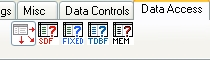
\includegraphics[width=0.3\textwidth]{Kapitel/datenbanken/pics/DataAccess}}
\label{fig:LazDataAccess01} F�r die Erstellung, Verwaltung und Zugriff auf Dbase und Foxpro Datenbanken ist die Komponenete 'TDBF' zust�ndig. F�r Datenbanken direkt im Speicher ist die Komponenete 'MEM', f�r Datenbanken mit eine festen Format (CSV) die Komponente 'FIXED' und Textbasierende Datens�tze mittels der Komponente 'SDF'.
F�r Serverdatenbanken sind die Komponenten auf der Seite 'SQLdb'\footnote{Siehe Kapitel \ref{SQLdb} auf Seite \pageref{SQLdb}} zu verwenden.

Die Komponente 'TDatasource' dient unter andern als Verbindung zu den grafischen Komponenten.

\subsection{TDatasource}

\subsection{SDF}
%  public
%    constructor Create(AOwner: TComponent); override;
%  published
%    property Delimiter: Char read FDelimiter write SetDelimiter;
%    property FirstLineAsSchema: Boolean read FFirstLineAsSchema write SetFirstLineAsSchema;
%  end;
%
\subsection{FIXED}
%  public
%    constructor Create(AOwner: TComponent); override;
%    destructor  Destroy; override;
%    function  GetFieldData(Field: TField; Buffer: Pointer): Boolean; override;
%    procedure RemoveBlankRecords; dynamic;
%    procedure RemoveExtraColumns; dynamic;
%    procedure SaveFileAs(strFileName : String); dynamic;
%    property  CanModify;
%    procedure LoadFromStream(Stream :TStream);
%    procedure SavetoStream(Stream :TStream);
%  published
%    property FileMustExist: Boolean read FFileMustExist write SetFileMustExist;
%    property ReadOnly: Boolean read FReadOnly write SetReadOnly;
%    property FileName : TFileName read FFileName write SetFileName;
%    property Schema: TStringList read FSchema write SetSchema;
%    property TrimSpace: Boolean read FTrimSpace write SetTrimSpace default True;
%    property FieldDefs;
%    property Active;
%    property AutoCalcFields;
%    property Filtered;
%    property BeforeOpen;
%    property AfterOpen;
%    property BeforeClose;
%    property AfterClose;
%    property BeforeInsert;
%    property AfterInsert;
%    property BeforeEdit;
%    property AfterEdit;
%    property BeforePost;
%    property AfterPost;
%    property BeforeCancel;
%    property AfterCancel;
%    property BeforeDelete;
%    property AfterDelete;
%    property BeforeScroll;
%    property AfterScroll;
%//    property BeforeRefresh;
%//    property AfterRefresh;
%    property OnCalcFields;
%    property OnDeleteError;
%    property OnEditError;
%    property OnFilterRecord;
%    property OnNewRecord;
%    property OnPostError;

\subsection{TDBF}

\subsection{MEM}
%\subsubsection{Datentypen}
%\begin{verbatim}
%   ftString :   result:=FieldDefs.Items[FieldNo-1].Size+1;
%   ftBoolean :  result:=SizeOf(Wordbool);
%   ftFloat :    result:=SizeOf(Double);
%   ftLargeInt : result:=SizeOf(int64);
%   ftSmallInt : result:=SizeOf(SmallInt);
%   ftInteger :  result:=SizeOf(Integer);
%   ftDate :     result:=SizeOf(TDateTime);
%   ftTime :     result:=SizeOf(TDateTime);
%   ftDateTime : result:=SizeOf(TDateTime);
%\end{verbatim}

%
%  public
%    constructor Create(AOwner:tComponent); override;
%    destructor Destroy; override;
%    procedure CreateTable;
%
%    Function  DataSize : Integer;
%
%    procedure Clear(ClearDefs : Boolean);
%    procedure Clear;
%    Procedure SaveToFile(AFileName : String);
%    Procedure SaveToFile(AFileName : String; SaveData : Boolean);
%    Procedure SaveToStream(F : TStream);
%    Procedure SaveToStream(F : TStream; SaveData : Boolean);
%    Procedure LoadFromStream(F : TStream);
%    Procedure LoadFromFile(AFileName : String);
%    Procedure CopyFromDataset(DataSet : TDataSet);
%    Procedure CopyFromDataset(DataSet : TDataSet; CopyData : Boolean);
%
%    Property Modified : Boolean Read FModified;
%
%  published
%    Property FileName : String Read FFileName Write FFileName;
%    property Filtered;
%    Property Active;
%    Property FieldDefs;
%    property BeforeOpen;
%    property AfterOpen;
%    property BeforeClose;
%    property AfterClose;
%    property BeforeInsert;
%    property AfterInsert;
%    property BeforeEdit;
%    property AfterEdit;
%    property BeforePost;
%    property AfterPost;
%    property BeforeCancel;
%    property AfterCancel;
%    property BeforeDelete;
%    property AfterDelete;
%    property BeforeScroll;
%    property AfterScroll;
%    property OnDeleteError;
%    property OnEditError;
%    property OnNewRecord;
%    property OnPostError;
%    property OnFilterRecord;
%  end;
\subsection{SQLite}
Diese Komponente ist standardm�ssig nicht vorhanden. Dazu mu� erst das Paket 'sqlite3laz 0.3'oder besser installiert werden.  \parpic[sl][r]{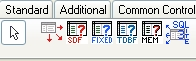
\includegraphics[width=0.3\textwidth]{Kapitel/datenbanken/pics/DataAccessLite}}
\label{fig:LazDataAccess02}Nach dem neu erstellen der IDE, befindet sich die Komponente hier.


%    function BookmarkValid(ABookmark: TBookmark): Boolean; override;
%    function CompareBookmarks(Bookmark1, Bookmark2: TBookmark): Longint; override;
%    function GetFieldData(Field: TField; Buffer: Pointer): Boolean; override;
%    function GetFieldData(Field: TField; Buffer: Pointer; NativeFormat: Boolean): Boolean; override;
%    function Locate(const KeyFields: string; const KeyValues: Variant; Options: TLocateOptions) : Boolean; override;
%    function LocateNext(const KeyFields: string; const KeyValues: Variant; Options: TLocateOptions) : Boolean;
%    function Lookup(const KeyFields: string; const KeyValues: Variant; const ResultFields: string): Variant;override;
%    // Additional procedures
%    function ApplyUpdates: Boolean;
%    function CreateTable: Boolean;
%    function CreateTable(const ATableName: String): Boolean;
%    procedure ExecCallback(const ASql: String; UserData: Pointer = nil);
%    procedure ExecSQLList;
%    procedure ExecuteDirect(const ASql: String);virtual;abstract;
%    procedure QueryUpdates(RecordStates: TRecordStateSet; Callback: TQueryUpdatesCallback; UserData: Pointer=nil);
%    function QuickQuery(const ASql:String):String;overload;
%    function QuickQuery(const ASql:String;const AStrList: TStrings):String;overload;
%    function QuickQuery(const ASql:String;const AStrList: TStrings;FillObjects:Boolean):String;virtual;abstract;overload;
%    procedure RefetchData;
%    function TableExists: Boolean;
%    function TableExists(const ATableName:String):Boolean;
%    function UpdatesPending: Boolean;
%    property ExpectedAppends: Integer read FExpectedAppends write SetExpectedAppends;
%    property ExpectedUpdates: Integer read FExpectedUpdates write SetExpectedUpdates;
%    property ExpectedDeletes: Integer read FExpectedDeletes write SetExpectedDeletes;
%    property IndexFields[Value: Integer]: TField read GetIndexFields;
%    property RowsAffected: Integer read GetRowsAffected;
%    property ReturnCode: Integer read FReturnCode;
%    property SqliteHandle: Pointer read FSqliteHandle;
%    property SqliteVersion: String read GetSqliteVersion;
%    property SQLList:TStrings read FSqlList;
%   published
%    property AutoIncrementKey: Boolean read FAutoIncrementKey write FAutoIncrementKey;
%    property IndexFieldNames: string read FIndexFieldNames write FIndexFieldNames;
%    property FileName: String read FFileName write SetFileName;
%    property OnCallback: TSqliteCallback read FOnCallback write FOnCallback;
%    property PrimaryKey: String read FPrimaryKey write FPrimaryKey;
%    
%    property TableName: String read FTableName write FTableName;   
%    property MasterSource: TDataSource read GetMasterSource write SetMasterSource;
%    property MasterFields: string read GetMasterFields write SetMasterFields;
%    
\subsubsection{ExecSQL}
\begin{description}
  \item \texttt{procedure ExecSQL(const ASql:String);}\\F�hrt den in ASql definierten String aus, liefert aber keine Datenmenge zur�ck.
  \item \texttt{procedure ExecSQL;}\\F�hrt die in der Eigenschaft SQL definierten SQL-Befehle aus, liefert aber keine Datenmenge zur�ck.
  \begin{description}
    \item Methode von TSqlite3Dataset
  \end{description}
\end{description}

\subsubsection{ApplyUpdates}
\begin{description}
  \item \texttt{function ApplyUpdates: Boolean;}\\�bertr�gt die �nderungen von der Datenmenge in die Datenbank.
  \begin{description}
    \item Methode von TSqlite3Dataset>TCustomSqliteDataset
  \end{description}
\end{description}

\subsubsection{ExecSQL}
\begin{description}
  \item \texttt{procedure ExecSQL(const ASql:String);}\\F�hrt den in ASql definierten String aus, liefert aber keine Datenmenge zur�ck.
  \item \texttt{procedure ExecSQL;}\\F�hrt die in der Eigenschaft SQL definierten SQL-Befehle aus, liefert aber keine Datenmenge zur�ck.
  \begin{description}
    \item Methode von TSqlite3Dataset
  \end{description}
\end{description}

\subsubsection{Active}
\begin{description}
  \item \texttt{property Active: Boolean read GetActive write SetActive default False;}\\ Sagt aus ob die Komponente derzeit aktiv ist und eine Datenmenge zur�ckliefert. Ein setzen auf 'true' entspricht der Methode 'Open' und ein setzen auf 'false' entspricht der Methode 'Close'.
  \begin{description}
    \item Eigenschaft von TSqlite3Dataset>TCustomSqliteDataset>TDataSet
  \end{description}
  \begin{description}
    \item Zugriff: Lesend und schreibend
    \item Defaultwert: false
  \end{description}
\end{description}

\subsubsection{SaveOnClose}
\begin{description}
  \item \texttt{property SaveOnClose: Boolean read FSaveOnClose write FSaveOnClose;}\\Wenn true, dann wird beim Schliessen der Datenmenge automatisch ein ApplyUpdates durchgef�hrt.
  \begin{description}
    \item Eigenschaft von TSqlite3Dataset>TCustomSqliteDataset
  \end{description}
  \begin{description}
    \item Zugriff: Lesend und schreibend
  \end{description}
\end{description}

\subsubsection{SaveOnRefetch}
\begin{description}
  \item \texttt{property SaveOnRefetch: Boolean read FSaveOnRefetch write FSaveOnRefetch;}\\Wenn true, dann wird vor dem Holen neuer Datenmengen automatisch ein ApplyUpdates durchgef�hrt.
  \begin{description}
    \item Eigenschaft von TSqlite3Dataset>TCustomSqliteDataset
  \end{description}
  \begin{description}
    \item Zugriff: Lesend und schreibend
  \end{description}
\end{description}

\subsubsection{SQL}
\begin{description}
  \item \texttt{property SQL: String read FSql write FSql;}\\In SQL befindet sich das SQL Statement was ausgef�hrt werden soll.
  \begin{description}
    \item Eigenschaft von TSqlite3Dataset>TCustomSqliteDataset
  \end{description}
  \begin{description}
    \item Zugriff: Lesend und schreibend
  \end{description}
\end{description}

\verb|Version: $$ |\footnote{ Autor: Andreas Frie�\\Lizenz: GFDL}
\newpage
%###########################################################
% Beispiele
%###########################################################
\chapter{Beispiele}
%--------------------------------------------------
% Sektion f�r Datenbank (MySQL,SQLlite,Firebird,..)
%--------------------------------------------------
\section[Datenbanken MySQL 5.x]{DatenbankenMySQL5x}
%%####################################################################
%    Copyright @ 2007 Andreas Frie� (Friess)
%    Permission is granted to copy, distribute and/or modify this document
%    under the terms of the GNU Free Documentation License, Version 1.2
%    or any later version published by the Free Software Foundation;
%    with no Invariant Sections, no Front-Cover Texts, and no Back-Cover Texts.
%    A copy of the license is included in the section entitled ``GNU
%    Free Documentation License''.
%%####################################################################
% Created: 17.08.2007
% @cvs($Date: 2007-09-05 19:46:18 +0000 (Wed, 05 Sep 2007) $)
% @cvs($Rev: 38 $)
% @cvs($Author: af0815 $)
% @cvs($URL: file:///svn/p/lazsnippets/code/trunk/dokumentation/LazSnippets/Kapitel/datenbanken/HowToNewMySQL.tex $)
%%####################################################################
\subsection{Demodatenbank MySQL}

%%####################################################################
\subsubsection{Installieren von MySQL 5.x}
Am einfachsten ist es im Internet auf die MySQL-Seite\footnote{http://www.mysql.de/} zu gehen und dort unter "`Community"'\footnote{http://dev.mysql.com/} den Punkt "`Downloads"' und "`MySQL Community Server"' auszusuchen. Dort kann man sich dann den entsprechenden Server f�r sein Betriebssystem aussuchen und herunterladen. Die Dateigr��e kann schon einen Breitband Internetzugang verlangen, denn je nach Version sind bis zu knappen 100 MB Download-Volumen gefragt.

Weiters ist es zu empfehlen, das man sich unter "`Downloads, GUI Tools"' auch noch die Programme "`MySQL Administrator"' und "`MySQL Query Browser"' herunterl�dt. Mit Hilfe der beiden Tools kann man sp�ter dann den Server komfortabel administrieren und auch die Datenbanken verwalten und Scripts laufen lassen. Die Tools sind nicht zwingend erforderlich, erleichtern aber gerade am Anfang das Leben. 

Eine Alternative dazu ist sicherlich auch das arbeiten mit "`PHPMySQLAdmin"'. Das Tool ist sehr ausgereift und auch entsprechend bekannt. Ein Nachteil dabei ist, das es einen Webserver mit PHP voraussetzt.

Zur Installation geht man entsprechend den Erfordernissen seines Betriebssystems vor. Es w�rde den Rahmen dieser Beschreibung sprengen, f�r jedes Betriebssystem mit seinen Eigenheiten eine entsprechende Anleitung zu erstellen.

Wichtig ist nur, das man bei der Installation  und Konfiguration nicht vergisst, ein gutes Passwort f�r den "`root"' ("`Administrationsuser"') zu w�hlen. Denn sp�ter vergisst man gerne den laufenden MySQL-Server und wenn der Rechner dann doch im Internet auftaucht, so hat man ein ganz sch�nes Sicherheitsleck, das einem gar nicht bewusst ist. Dasselbe gilt nat�rlich in abgemilderter Form auch f�r normale Benutzer, die etwas mehr Rechte als lesen in der Datenbank haben. Eine gute M�glichkeit ist, ein launiges Sprichwort zu nehmen und die Anfangsbuchstaben aneinander zu reihen. Beispiel: "`Wir sind ja nicht bl�d Mann und haben 99 Luftballone gekauft"'. Daraus kann sich ein Pa�wort wie folgt ergeben "`WsjnbMuh99Lg"'. Das l�sst sich noch so halbwegs merken und besteht aus Gro�\- und Kleinbuchstaben, beinhaltet Zahlen und ist au�erdem noch zw�lf Zeichen lang. 

Aber genug dem Ausflug in die Installation und Pa�wortauswahl, beginnen wir nun mit der Erstellung unserer Datenbank, die sich dann sp�ter durch alle Beispiele ziehen wird.

%%####################################################################
\subsubsection{Erstellung der DEMO Datenbank}
Das Erste, das wir am neuen oder geleerten MySQL Datenbankserver erstellen, ist eine neue Datenbank f�r unsere Zwecke. Dazu �ffnen wir den "`MySQL Query Browser"'.
\parpic[sl][r]{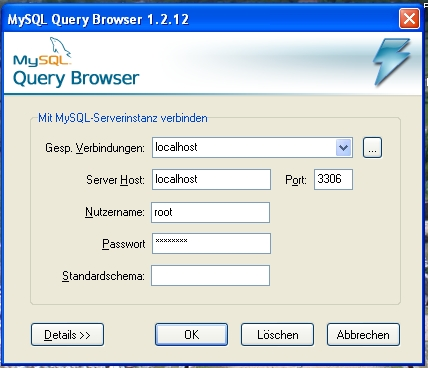
\includegraphics[width=0.3\textwidth]{Kapitel/datenbanken/pics/NewDB01}}
%\parpic[lf][r]{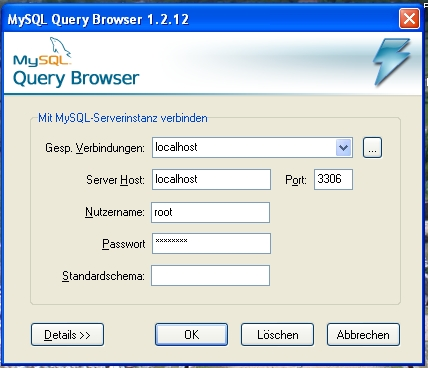
\includegraphics[width=6cm,height=6cm]{Kapitel/datenbanken/pics/NewDB01}}
%\caption[NewDB01]{Verbindungsdialog}
\label{fig:NewDB01}
%\begin{figure}[tp]
%\centering
%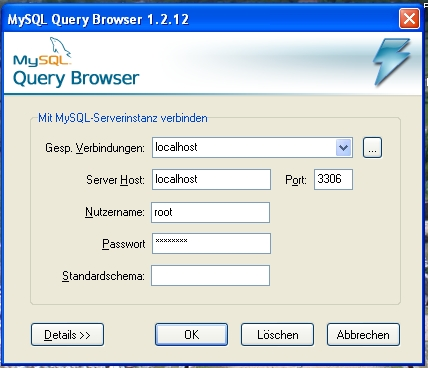
\includegraphics[totalheight=0.3\textwidth]{Kapitel/datenbanken/pics/NewDB01}
%\caption[NewDB01]{NewDB01}
%\label{fig:NewDB01}
%\end{figure}
Es �ffnet sich als ersters das Verbindungsfenster. Ich werde jetzt die Felder von oben nach unten besprechen, denn es k�nnte ja sein, das sie eine andere Sprachversion verwenden. 

Unter "`Gesp. Verbindungen"' wird ein beliebiger Namen eingetragen, unter der sp�ter die Einstellungen wieder abgerufen werden k�nnen. Bei "`Server Host"' und "`Port"' geben wir, bei einer lokalen Installation, "`localhost"' und "`3306"' ein. Wobei die Portnummer "`3306"' der Standardport von MySQL ist. Als n�chstes kommen jetzt der "`Nutzername"' und das "`Passwort"' dran, dort geben wir in diesem Fall den Benutzer "`root"' mit dem bei der Installation vergebenen Pa�wort ein. Sp�ter sollte man sich nur in zwingend notwendigen F�llen mit dem Administratorpa�wort verbinden. Das Feld "`Standardschema"' lassen wir bei diesem ersten Einstieg einmal leer.
\parpic[sr][r]{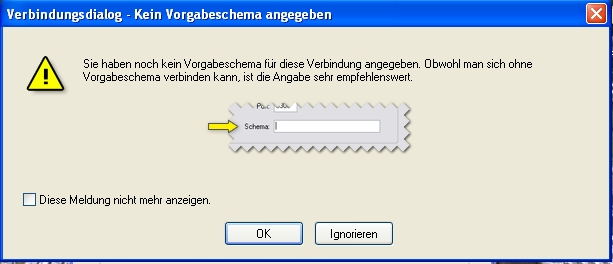
\includegraphics[width=0.3\textwidth]{Kapitel/datenbanken/pics/NewDB02}}
%\caption[NewDB02]{Fehlendes Standardschema}
\label{fig:NewDB02}

Anschliessend gehen wir mit "`Ok"' im Dialog weiter, das nun folgende Hinweisfenster zum Thema fehlendes Standardschema �bergehen wir mit dem Button "`Ignorieren"'. Ist bis jetzt alles gut verlaufen und der MySQL Datenbakserver aktiv, so �ffnet sich jetzt endg�ltig der "`MySQL Query Browser"'.

\parpic[sl][r]{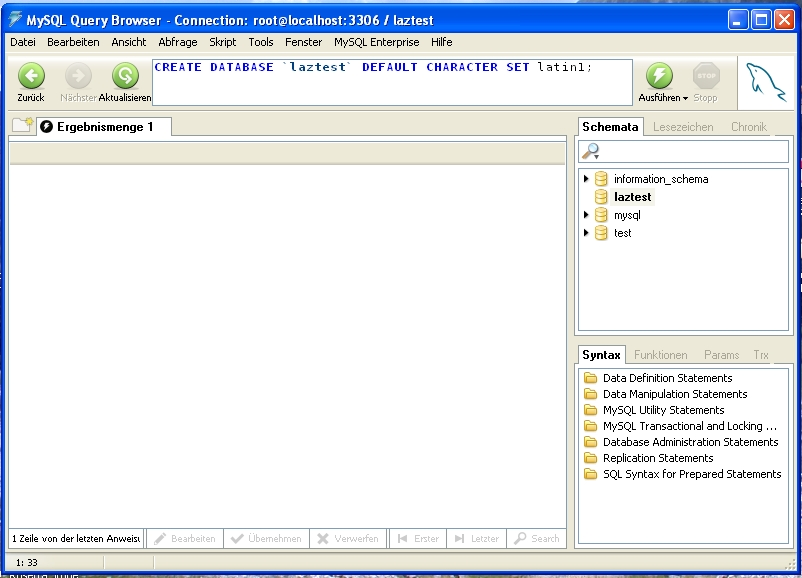
\includegraphics[width=0.3\textwidth]{Kapitel/datenbanken/pics/NewDB03}}
\label{fig:NewDB03}
Als ersters erzeugen wir mittels \textbf{\emph{CREATE USER lazarus@localhost IDENTIFIED BY 'WsjnbMuh99Lg';}} einen neuen Benutzer, der noch dazu ein halbwegs sicheres Pa�wort hat. Zus�tzlich geben wir diesen Benutzer alle Recht an dieser Datenbank mit folgenden Befehl \textbf{\emph{GRANT all ON *.* TO lazarus@localhost;}}. Somit hat der Benutzer alle Rechte au�er dem Recht, selbst Rechte zu vergeben.

Im Men�punkt "`Datei"' w�hlen wir die Funktion "`Verbindung umschalten"' an und wechseln die Verbindung auf den User "`lazarus@localhost"'. Alternativ kann man den "`MySQL Query Browser"'  schliessen und als Benutzer "`lazarus"' neu anmelden. Damit wir nicht immer die Informationen neu eingeben m�ssen, kann man den Button rechts neben den "`Gesp. Verbindungen"' benutzen und sich dort ein entsprechndes Profil anlegen. Somit braucht man sp�ter nur sein Profil in der Top-Down Box anw�hlen, das Pa�wort eingeben und schon ist man drinnen. 

Anschlie�end erzeugen wir jetzt als Benutzer "`lazarus@localhost"' mittels dem Kommando \textbf{\emph{CREATE DATABASE `laztest` DEFAULT CHARACTER SET latin1;}} eine neue Datenbank, mit dem Namen "`laztest"'. Diese Zeile geben wir oben im "`MySQL Query Browser"' ein und dr�cken dann auf den gr�nen Button daneben. Anschlie�end k�nnen wir mit der Maus auf "`Schemata"' klicken und mit der Taste "`F5"' ein neuerliches einlesen der �bersicht der Datenbanken (= Schemata) erreichen. Jetzt sollte dort unsere neue Datenbank vorhanden sein.  

Somit haben wir die Datenbank erstellt und auch einen Beutzer mit hohen Rechten darin erzeugt. F�r den produktiven Betrieb w�rde sich jetzt noch anbieten, einen Benutzer zu erzeugen, der entsprechend den Erfordernissen weniger Rechte hat. Aber nachdem das hier ja ein Tutorium ist, belassen wir es einmal dabei.

\subsubsection{Windows FAQ}
\paragraph{Einleitung}
Es hat sich auch bei mir gezeigt, das es manchmal nicht so einfach ist, MySQL unter Lazarus zu verbinden. Hier ein paar Hilfen.

\paragraph{Cannot load MySQL library "`libmysql.dll"'}
Dieser Fehler kann mehrer Ursachen haben. Die einfachste ist, dass auf dem Rechner ganz einfach die Treiber f�r MySQL nicht installiert sind. 
\parpic[sr][r]{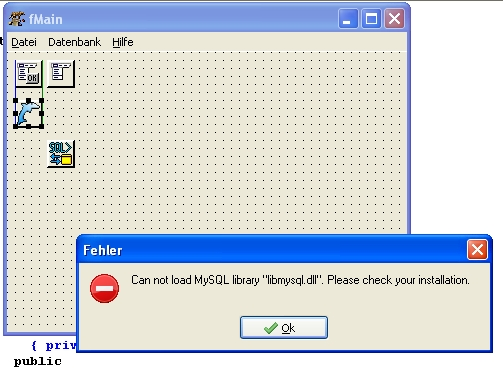
\includegraphics[width=0.3\textwidth]{Kapitel/datenbanken/pics/FAQWDB01}}
\label{fig:FAQWDB01}
Die Abhilfe ist die Datei in ein Verzeichnis, dass sich im Suchpfad befindet zu kopieren. Genauso ist es m�glich, die Bibliothek ins selbe Verzeichnis wie die ausf�hrbare Datei zu kopieren, der Weg bietet sich an, wenn es an den Rechten am Systemverzeichnis fehlt.

Wenn das ganze, wie am Bild, innerhalb von Lazarus passiert, so kann es einmal am Lazarus liegen. Besonders wenn man eine Version aus dem SVN selbst kompiliert, kann es vorkommen, das es hier Probleme gibt. Die Abhilfe ist nur, eine bessere oder stabile Version von Lazarus zu verwenden. 
Genauso kann es sein, dass wie oben bereits besprochen, die Biblothek fehlt. Die Abhilfe ist wieder die Biblothek in ein Verzeichnis, dass im Suchpfad liegt zu kopieren. Geht das nicht, so mu� die Datei einmal in des Verzeichnis kopiert werden, wo sich die "`Lazarus.exe"' befindet und einmal in das Verzeichnis, wo die ausf�hrbare Datei des Projektes liegt. Denn innerhalb der IDE ben�tigt Lazarus die Datei in seinem Pfad, wird die Datei aber ausgef�hrt, so ben�tigt sie das aktuelle, kompilerte und gestartete Programm.

\verb|Version: $LastChangedRevision: 38 $ |\footnote{ Autor: Andreas Frie�\\Lizenz: GFDL}

%%####################################################################
%    Copyright @ 2007 Andreas Frieß (Friess)
%    Permission is granted to copy, distribute and/or modify this document
%    under the terms of the GNU Free Documentation License, Version 1.2
%    or any later version published by the Free Software Foundation;
%    with no Invariant Sections, no Front-Cover Texts, and no Back-Cover Texts.
%    A copy of the license is included in the section entitled ``GNU
%    Free Documentation License''.
%%####################################################################
% Created: 21.08.2007
% @cvs($Date: 2007-09-05 19:46:18 +0000 (Wed, 05 Sep 2007) $)
% @cvs($Rev: 38 $)
% @cvs($Author: af0815 $)
% @cvs($URL: file:///svn/p/lazsnippets/code/trunk/dokumentation/LazSnippets/Kapitel/datenbanken/ProjektMySQLSimple.tex $)
%%####################################################################
\subsection{Projekt MySQLSimple}
\paragraph{Einleitung}
In diesem Projekt wird nur eine einfache Verbindung zur Datenbank aufgebaut und die grundlegenden Elemente die dafür notwendig sind erklärt. Es werden hierbei nur Elemente verwendet die bei einer Standardinstallation von Lazarus dabei sind.

\paragraph{Datenbank}
In der Datenbank muß für dieses Beispiel folgende Anweisung ausgeführt werden oder das ganze mittels des "`MySQL Query Browser" erstellt werden.
\begin{verbatim}
CREATE TABLE `laztest`.`ST_Person` (
  `STPerson` INTEGER UNSIGNED NOT NULL AUTO_INCREMENT \
     COMMENT 'Primaerschluessel',
  `cVName` VARCHAR(45) NOT NULL DEFAULT '' COMMENT 'Vorname',
  `cFName` VARCHAR(45) NOT NULL DEFAULT '' COMMENT 'Familienname',
  `cMName` VARCHAR(15) NOT NULL DEFAULT '' COMMENT 'Namensergaenzung',
  `cRName` VARCHAR(45) NOT NULL DEFAULT '' COMMENT 'Rufname',
  PRIMARY KEY (`STPerson`),
  UNIQUE INDEX `Namen_idx`(`cVName`, `cFName`, `cRName`)
)
ENGINE = InnoDB
CHARACTER SET latin1 COLLATE latin1_german1_ci
COMMENT = 'Personendaten';
\end{verbatim}
Wir erstellen hier einmal die für das Beispiel notwendige Tabelle für Personendaten. 
\parpic[sr][l]{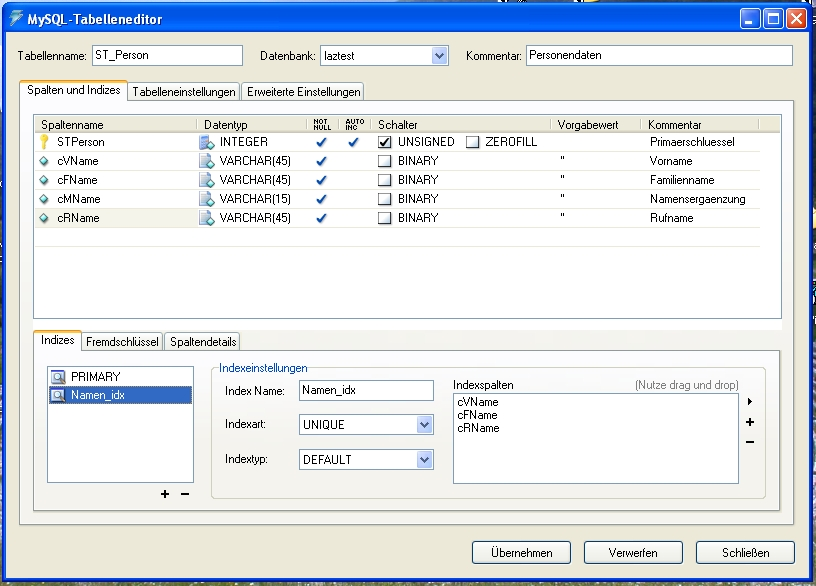
\includegraphics[width=0.35\textwidth]{Kapitel/datenbanken/pics/MySQLSimple02}}
\label{fig:MySQLSimple02}
Warum habe ich den Namen "`ST\_Person"' gewählt. Ganz einfach, ich rechne Tabellen mit diesem Inhalt zu den so genannten Stammdatentabellen. Das stimmt, außer wir haben hier eine reine Personenverwaltung. Nachdem das Beispiel aber erwitert werden soll, werden auch noch andere Tabellen folgen. 

Wir verwenden hier einmal die Spalte "`STPerson"' für den nicht Null  beinhaltenden (NOT NULL), automatisch hochzählenden (AUTO\_INCREMENT), eindeutigen Primärschlüssel (PRIMARY KEY ('STPerson')). In der Spalten "`cVName"' und "`cFName"' kommen der Vorname und der Familienname (=Nachname) hinein, zusätzlich gibt es noch das Feld für einen eventuelle Namensergänzung. Weiters beinhaltet die Spalte "`cRName"' noch den Rufnamen der Person.

Fast ganz unten in der definition der Tabelle befindet sich ein Hinweis auf einen weiteren Index. Dieser eindeutige Index (UNIQUE INDEX) soll verhindern, das gleiche Personen mehrmals in der Tabelle angelegt werden können. Warum wird dann aber nicht nur die Felder des Vornamens und des Familienanmens herangezogen ? Na, ja, was ist wenn wir mehrere "`Max Mustermann"' haben ! Im richtigen Leben hat man dann ja selbst noch hilfen, das zu unterscheiden. Dazu dient der Rufname (= Spitzname). Denn dann kannman den "`Max aus D"' und den "`Max aus A"' auch noch eintragen und die EInträge sind jetzt trotz der Namensgleichheit wirklich auseinander zu halten.

\paragraph{Benutzerschnittstelle}
Die Komponeneten kommen von der Palettenseite "`SQLdb"', "`DataAccess"' und "`DataControls"'.
\parpic[sr][l]{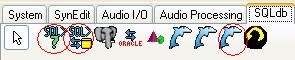
\includegraphics[width=0.35\textwidth]{Kapitel/datenbanken/pics/MySQLSimple01A}} \label{fig:MySQLSimple01A} 
Fangen wir einmal mit der "`SQLdb"' an. Um auf eine Datenbank zugreifen zu können, benötigen wir einmal eine Verbindungskomponente, das ist in unseren Fall eine der zur Datenbank passende Connection (= Verbindung). Da wir einen MySQL Server 5.x am laufen haben, so nehmen wir die passende "`MySQL50Connection"' Komponente und bringen sie auf das Projekt.
\parpic[sr][l]{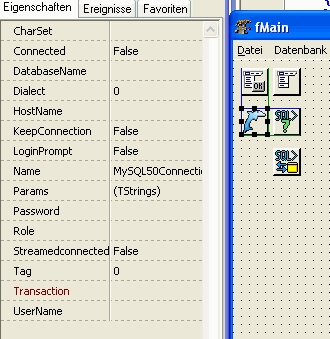
\includegraphics[width=0.25\textwidth]{Kapitel/datenbanken/pics/MySQLSimple03}} \label{fig:MySQLSimple03} 
Weiters fügen wir noch eine "`TSQLTransaction"' Komponente unserer Form hinzu.

Jetzt der Reihe nach, angefangen bei der "`TMySQL50\-Connection"' Komponente, müssen wir Einstellungen im Objektinspektor treffen. 

Bei der "`TMySQL50Connection"' Komponente sind es folgene Einstellungen. Der \textbf{DatabaseName} wird auf den Namen unserer Datenbank \emph{laztest} gesetzt. Der \textbf{HostName} ist bei einer kokalen installation immer \emph{localhost}. Für das \textbf{Paßwort} nehmen wir das des Benutzers, der sich mit der Datenbank verbindet. Bei \textbf{Transaction} müssen wir nur in das im Objektinspektor klicken und eine Auswahl erscheint. Wir nehmen hier unsere \emph{SQLTransaction1}. Als letztes geben wir den \textbf{UserNamen} ein, das ist ganz einfach der Benutzer den wir in der Datenbank erstellt haben, also \emph{lazarus@localhost}.

Die nächste Komponenete ist die "`TSQLTransaction"'. Dort müssen wir aktuell nichts einstellen, da sich die Eigenschaft \textbf{Database} im Objektinspektor bereits selbst auf \emph{MySQL50Connection1} geändert hat.

Den ersten Test kann man jetzt bereits durchführen. Durch anklicken der Eigenschaft \textbf{Connected} von \textbf{MySQL50Connection1} wechselt diese von \emph{False} auf \emph{True}. Wenn alles gut gelaufen ist, so läuft die Verbindung ohne Probleme ab. Wenn nicht, so muß man die Einstellungen nochmals überprüfen. Anschliessen stellen wir die Eigenschaft wieder auf \emph{False} zurück.

Nachdem die Verbindung zur Datenbank möglich ist, so müssen wir jetzt die Komponeneten für die Abfrage der Datenbank und die Anzeige der Daten noch hinzufügen. Es handelt sich hier um die Komponeneten "`TSQLQuery"' von Tab "`sqldb"', "`TDataSource"' vom Tab "`Data Access"' und "`TDBGrid"' vom Tab "`Data Controls"'.

Fangen wir mit der Komponente "`SQLQuery1"' an. Sie ist zuständig für die richtige Abfrage am Datenbankserver. Wir stellen die Eigenschaft \textbf{DataBase} auf unsere \emph{MySQL50Connection1} ein. Weiters müssen wir in die Eigenschaft \textbf{SQL} folgendes einfügen
\begin{verbatim}
SELECT `STPerson`, `cVName`, 
       `cFName`, `cMName`, `cRName`
  FROM st_person;
\end{verbatim}
und den Eigenschaftseditor wieder schließen. Die Eigenschaft hat sich \textbf{Transaction} im Objektinspektor bereits selbst auf \emph{SQLTransaction1} geändert. In der Komponenete "`Datasource1"' müssen wir nur \textbf{DataSet} per Mausklick auf \emph{SQLQuery1} einstellen. Als letztes konfigurieren wir das "`TDBGrid"'. Wir ändern mit der Maus die Eigenschaft \textbf{Align} auf \emph{alClient} und die Eigenschaft \textbf{DataSource} auf \emph{Datasource1}. Damit erfasst das Grid das komplette Formular. 

Prinzipiell ist unser Programm jetzt einmal optisch fertig. Wenn wir es jetzt kompilieren und laufen lassen, sehen wir das Formular, aber keine Daten und ändern können wir auch nichts. Es ist klar, wir haben die Komponenten konfiguriert, aber etwas Code wird auch benötigt um den Komponenten zu sagen, was wir wirklich wollen.

Dazu verwenden wir eine "`TActionList"' und ein "`TMainmenu"' aus dem Tab "`Standard"'. In der \textbf{ActionList1} erzeugen wir ganz einfach die Ereignisse \emph{actCloseDB}, \emph{actOpenDB} und \emph{actDataSetRefresh}. Ausserdem Erzeugen wir die Ereignisproceduren für das Form erzeugen un Form schliessen. Im MainMenu Komponente erzeugen dann ein kleines Menü.

\begin{verbatim}
procedure TfMain.actOpenDBExecute(Sender: TObject);
begin
  if not MySQL50Connection1.Connected then
  begin
    MySQL50Connection1.Connected := true;
  end;
  if not SQLQuery1.Active then SQLQuery1.Active := true;
end;
\end{verbatim}
Beim Eintreffen des Ereignisses für das Öffnen der Datenbank, wird als erstes Abgefragt ob die Verbindung bereits besteht. Ist die Verbindung vorhanden, so wird die Abfrage selbst geöffnet, falls sie noch nicht offen war.

\begin{verbatim}
procedure TfMain.actCloseDBExecute(Sender: TObject);
begin
  if MySQL50Connection1.Connected then
  begin
    if SQLQuery1.Active then
    begin
      SQLQuery1.ApplyUpdates;
      SQLQuery1.Active := false;
    end;
    MySQL50Connection1.Connected := false;
  end;
end;
\end{verbatim}
Wenn die Datenbank wieder geschlossen werden soll, so sind zuerst die noch nicht gespeicherten Daten zurückzuschreiben, dies geschieht mit dem Kommando \emph{ApplyUpdates}. Ohne diese Kommando bleiben die Änderungen nur lokal und werden mit der nächsten Abfrage wieder überschrieben. Anschliessend wird die Abfrage deaktiviert, dannach die Verbindung.

\begin{verbatim}
procedure TfMain.actDataSetRefreshExecute(Sender: TObject);
begin
  if not SQLQuery1.Active then exit;
  SQLQuery1.ApplyUpdates;
  SQLQuery1.Refresh;
end;
\end{verbatim}
Bei einer einfachen Auffrischung der Daten, arbeiten wir hier vorsichtshalber die Änderungen ein, bevor wir die eigentliche Auffrischung durchführen. Falls die Abfrage nicht aktiv war, brauchen wir klarerweise gar nichts zu machen.

\begin{verbatim}
procedure TfMain.FormDestroy(Sender: TObject);
begin
  actCloseDBExecute(Sender);
end;
\end{verbatim}
Wichtig ist, das beim Schließen des Formular, die Datenbankkomponenten wieder ordnungsgemäß von der Datenbank getrennt werden, ansonsten hat man Fehlermeldungen und auch blockierte Datenverbindungen. Generell sollte danch getrachtet werden, die Verbindungen, egal was geschieht, in konsistenten Zustand zu hinterlassen.

\paragraph{SVN}
Den Quelltext des Beispiel kann man sich auch mit folgenden Kommando aus dem SVN ind das aktuelle Verzeichnis holen.
\begin{verbatim}
svn co https://lazsnippets.svn.sourceforge.net/svnroot/lazsnippets/\
  trunk/datenbank/MySQL/MySQLSimple .
\end{verbatim}
Die Zeile ist in einem zu schreiben und wurde nur aus Formatierungsgründen hier beim Rückstrich (Backslash) umgebrochen. Der Punkt am Ende der Zeile ist notwendig, da es das Kennzeichen für das aktuelle Verzeichnis ist. Weiter ist auf die Schreibweise zu achten, das hier die Server zwischen Großbuchstaben und Kleinbuchstaben unterscheiden.
Die Datenbank muß man aber trotzdem selbst am MySQL Server erstellen. Die dazu benötigten Informationen befinden sich im Text von "`Datenbank"' weiter oben.

\paragraph{Version}
Derzeit ist das Beispiel mit der Version 0.9.23 beta von Lazarus entwickelt.
\begin{table}[htbp]
%	\centering
		\begin{tabular}[ht]{|l|l|}
      \hline
      Betriebssystem & getestet \\
      \hline
%      Linux Unbuntu & nein \\
      Linux Suse & nein \\
%      Linux Debian & nein \\
%      Win95 + WinME & nein \\
%      Win2k & nein \\
      WinXP & ja \\
%      WinVista & nein \\
      \hline
		\end{tabular}
\end{table}
\caption{Versionsübersicht}
\label{tab:MySQLSimpleVersion01} 

\verb|Version: $LastChangedRevision: 38 $ |\footnote{ Autor: Andreas Frieß\\Lizenz: GFDL}
\newpage
%%####################################################################
%    Copyright @ 2007 Andreas Frieß (Friess)
%    Permission is granted to copy, distribute and/or modify this document
%    under the terms of the GNU Free Documentation License, Version 1.2
%    or any later version published by the Free Software Foundation;
%    with no Invariant Sections, no Front-Cover Texts, and no Back-Cover Texts.
%    A copy of the license is included in the section entitled ``GNU
%    Free Documentation License''.
%%####################################################################
% Created: 28.08.2007
% @cvs($Date: 2007-09-05 19:46:18 +0000 (Wed, 05 Sep 2007) $)
% @cvs($Rev: 38 $)
% @cvs($Author: af0815 $)
% @cvs($URL: file:///svn/p/lazsnippets/code/trunk/dokumentation/LazSnippets/Kapitel/datenbanken/ProjektMySQLTestData.tex $)
%%####################################################################
\subsection{Projekt MySQLTestData}
\paragraph{Einleitung}
Es soll zeigen, wie man relativ einfach Testdaten in größerer Zahl in die Tabelle ST\_Person unserer Datenbank einfügt. Zugleich kann man es als Basis für Versuche mit SELECT Statements verwenden. In der Tabelle werden Lösch-, Einfüge- und Auswahloperationen durchgeführt.

\paragraph{Datenbank}
Es wird die Datenbank und Tabelle vom Beispiel \textbf{MySQLSimple} verwendet. Weitere Informationen können dort gefunden werden.

\paragraph{Benutzerschnittstelle}
Auf der Oberfläche befinden sich links drei Buttons. 
\parpic[sr][l]{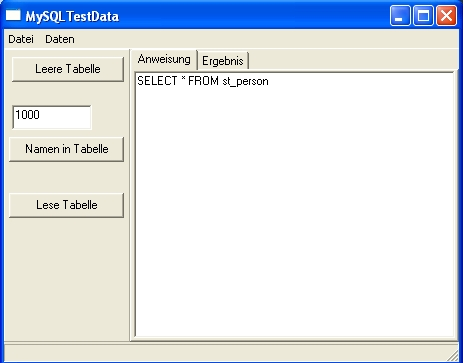
\includegraphics[width=0.25\textwidth]{Kapitel/datenbanken/pics/MySQLTestData01}} 
\caption{Projekt TestData GUI}
\label{fig:MySQLTestData01} 
Mit dem obersten Button wird die Tabelle komplett geleert, diese wird durch eine \emph{Delete} Anweisung im Quelltext durchgeführt. 
Der mittlere Button und das Eingabefeld darüber gehören zusammen und fügen neue Datensätze in der Tabelle ein. Die Anzahl der Datensätze wird durch den Wert im Eingabefeld vorgegeben.
Der unterste Button und das Tab-Sheet rechts daneben diesen zum Abfragen der Daten. Auf der ersten Seite des Tab-Sheets kann man das Abfrage Statement eingebn, die Anzeige erfolgt auf der zweiten Seite des Tab-Sheet.

Und jetzt die Funktionen mit den dahinterliegenden Code im Detail.
\subparagraph{Oberer Button}
Zuerst wird geprüft ob die Verbindung (Connection) zur Datenbank besteht, wenn nicht so wird die Verbindung hergestellt. Die Verbindungseinstelllungen wurden über den Objektinspektor schon beim Design getroffen, da es sich hier um Beispiele handelt.

\begin{verbatim}
if not MySQL50Connection1.Connected then
  MySQL50Connection1.Connected := true;
aSqlQuery := TSQLQuery.Create(self);
try
  aSqlQuery.SQL.Clear;
  aSqlQuery.DataBase := MySQL50Connection1;
  aSQLQuery.Transaction := SQLTransaction1;
  aSqlQuery.SQL.Add('DELETE FROM st_person;');
  aSqlQuery.ExecSQL;
finally
  aSqlQuery.free;
end;
\end{verbatim}

Anschliessend wird zur Laufzeit die TSQLQuery Komponente erzeugt. Wichtig ist, daß das Objekt erzeugt wird \verb|(aSqlQuery := TSQLQuery.Create(self);)|. Durch \emph{self} wird das Objekt dem Formular zugeordnet, so das das Formular beim Beenden auch das Objekt zerstören kann, falls es bis dahin noch nicht zerstört wurde.

Im nächsten Schritt wird ein eventuell vorhandenes gespeichertes SQL-Statement sicherheitshalber gelöscht. Weiters die Verbindung und die Transaktion zugewiesen. Dies geschieht genauso als würde man es über den Objektinspektor machen. Dann wird das neue SQL-Statement hinzugefügt. Da es ohne 'WHERE' EInschränkung verwendet wird, löscht es somit \textbf{alle} Daten aus der Tabelle. 

Zum Abschluß wird das verwendete SQL-Query Objekt wieder sauber entfernt. Damit dies auch geschieht wenn es einen Fehler gegeben hat, sind die Teile ab der Erstellung des Objektes durch ein try..finally Statement geklammert. Damit wird erreicht, das das Objekt auch nach einem Fehler richtig gelöscht wird.
\subparagraph{Mittlerer Button}
Beim betätigen des Buttons wird als erstes die Eingabe des Editfeldes überprüft und nur wenn der Wert in eine Zahl umgewndelt werden kann, wird fortgefahren.
\begin{verbatim}
try
  iAnzahl := StrToInt(edAnzahl.Text);
except
  showmessage('Nur Zahlen erlaubt');
  exit;
end;
\end{verbatim}

Mittels des Behfels \emph{randomize} wird der Zufallszahlengenerator initialisiert, dann die Verbindung zur Datenbank nötigenfalls hergestellt. Anschliessend eine TSQLQuery zur Laufzeit erzeugt und mit den nötigen Informationen versorgt.
\begin{verbatim}
randomize();
if not MySQL50Connection1.Connected then 
  MySQL50Connection1.Connected := true;
  
aSqlQuery := TSQLQuery.Create(self);
try
  aSqlQuery.SQL.Clear;
  aSqlQuery.DataBase := MySQL50Connection1;
  aSQLQuery.Transaction := SQLTransaction1;
\end{verbatim}
Weil wir später in einer Schleife Daten in die Datenbank einfügen, so erzeugen wir hier jetzt die nötigen Parameter. 

\textbf{HINWEIS:} Das Arbeiten mit Parametern ist wesentlich besser, als das Statement mittels Stringverwaltung zusammen zu setzen. Man vermeidet damit Probleme mit speziellen Zeichen, wie Hochkomma und der SQL-Server hat die Möglichkeit das Statement vor zu kompilieren und zu optimieren.

Anschliessend wird das SQL-Statement in die Query eingefügt. Mit den Doppelpunkt zeigt man, das es sich hier um einen Parameter handelt. 
\begin{verbatim}
  aSqlQuery.Params.CreateParam(ftInteger,'vname',ptInput);
  aSqlQuery.Params.CreateParam(ftInteger,'fname',ptInput);
  aSqlQuery.Params.CreateParam(ftInteger,'mname',ptInput);
  aSqlQuery.Params.CreateParam(ftInteger,'rname',ptInput);
  aSqlQuery.SQL.Add('INSERT st_person (cVName,cFName,cMName, cRName)');
  aSqlQuery.SQL.Add(' VALUES (:vname,:fname,:mname, :rname);');
\end{verbatim}
Hier beginnt die Schleife. ALs erstes werden dir Stringvariablen erzeugt, anschliessend die Strings den Parameteren übergeben.
\begin{verbatim}
  for i := 1 to iANzahl do
  begin
    iZufall := Random(MaxVorNamen-MinVorNamen) + MinVorNamen;
    cVName := VorNamen[iZufall];
    if cVName = '' then continue;

    iZufall := Random(MaxFamilienNamen-MinFamilienNamen) + 
                 MinFamilienNamen;
    cFName := FamilienNamen[iZufall];
    if cFName = '' then continue;

    cMName := leftStr(cVName,2)  +LeftStr(cFName,2);
    cRName := cVName + IntToStr(Random(10)) + cFName;

    aSqlQuery.Params.ParamByName('vname').AsString := cVName;
    aSqlQuery.Params.ParamByName('fname').AsString := cFName;
    aSqlQuery.Params.ParamByName('mname').AsString := cMName;
    aSqlQuery.Params.ParamByName('rname').AsString := cRName;
\end{verbatim}
Jetzt wird die Query mit den aktuellen Parametern durchgeführt. Der Befehl lautet \emph{ExecSQL}, dieser erwartet keine Ergebnismenge zurück. Das ist auch der Grund warum hier kein \emph{Open} oder \emph{Active=true} verwendet wurde, denn dieses erwarted das eine Ergebnismenge zurück geliefert wird. Anschliessend wird solange in der Schleife verblieben, bis alles abgearbeitet wurde. Wenn beim Ausführen ein Fehler auftritt, so wird in der Statuszeile eine Fehlermeldung angezeigt und mit dem nächsten durchlauf weitergemacht.
\begin{verbatim}
    try
      aSqlQuery.ExecSQL;
    except
      Statusbar1.SimpleText := 'Fehler in: ' + IntToStr(i);
      sleep(100);
    end;
  end;
finally
  aSqlQuery.free;
end;
\end{verbatim}

\subparagraph{Unterer Button}
Zum Unterschied vorher, ist diese Query zur Designzeit auf dem Formular hinterlegt worden. Damit entfällt das erzeugen zur Laufzeit. Das soll auch den Unterschied zwischen den beiden Methoden zeigen.

Es wird zuerst die Query inaktiv gemacht, falls sie offen war. Dann ganz einfach der Inhalt der Strings aus dem Meno in die Query übertragen und die Query wieder aktiv gemacht. Deshalb aktiv gemacht, da wir ja eine Ergebnismenge erwarten. Das hätten wir beim ausführen von \emph{ExecSQL} nicht.
\begin{verbatim}
  if SQLQuery1.Active then SQLQuery1.Active := false;
  SQLQuery1.SQL.Clear;
  SQLQuery1.SQL.Assign(Memo1.Lines);
  try
    SQLQuery1.Active := true;
  except
    showmessage('Anweisungen nicht gültig');
  end;
\end{verbatim}
Dann kann man im Datengitter die Ergebnisse betrachten.


\paragraph{SVN}
Den Quelltext des Beispiel kann man sich auch mit folgenden Kommando aus dem SVN ind das aktuelle Verzeichnis holen.
\begin{verbatim}
svn co https://lazsnippets.svn.sourceforge.net/svnroot/lazsnippets/\
  trunk/datenbank/MySQL/MySQLTestData .
\end{verbatim}
Die Zeile ist in einem zu schreiben und wurde nur aus Formatierungsgründen hier beim Rückstrich (Backslash) umgebrochen. Der Punkt am Ende der Zeile ist notwendig, da es das Kennzeichen für das aktuelle Verzeichnis ist. Weiter ist auf die Schreibweise zu achten, das hier die Server zwischen Großbuchstaben und Kleinbuchstaben unterscheiden.

\paragraph{Version}
\begin{table}[htbp]
%	\centering
		\begin{tabular}[ht]{|l|l|}
      \hline
      Betriebssystem & getestet \\
      \hline
%      Linux Unbuntu & nein \\
      Linux Suse & nein \\
%      Linux Debian & nein \\
%      Win95 + WinME & nein \\
%      Win2k & nein \\
      WinXP & ja \\
%      WinVista & nein \\
      \hline
		\end{tabular}
\end{table}
\caption{Versionsübersicht}
\label{tab:MySQLTestDataVersion01} 

\verb|Version: $LastChangedRevision: 38 $ |\footnote{ Autor: Andreas Frieß\\Lizenz: GFDL}

\newpage
\section[Datenbanken SQLite 3.x]{DatenbankenSQLite3x}
% "`Comming Soon"' af0815
%\input{Kapitel/datenbanken/HowToNewSQLite}
%\newpage
%\input{Kapitel/datenbanken/ProjektSQLiteSimple}
%\newpage
%\input{Kapitel/datenbanken/ProjektSQLiteTestData}

\section[Datenbanken DBase, FoxPro]{DatenbankenTDBF}
% "`Comming Soon"' af0815
%\input{Kapitel/datenbanken/HowToNewTDBF}
%\newpage
%\input{Kapitel/datenbanken/ProjektTDBFSimple}
%\newpage
%\input{Kapitel/datenbanken/ProjektTDBFTestData}

\newpage
\chapter{Programme}
%###############################################
% Kapitel f�r Tools
%###############################################
\section[N�tzliche Werkzeuge]{N�tzliche Werkzeuge}
%%####################################################################
%    Copyright @ 2007 Andreas Frieß (Friess)
%    Permission is granted to copy, distribute and/or modify this document
%    under the terms of the GNU Free Documentation License, Version 1.2
%    or any later version published by the Free Software Foundation;
%    with no Invariant Sections, no Front-Cover Texts, and no Back-Cover Texts.
%    A copy of the license is included in the section entitled ``GNU
%    Free Documentation License''.
%%####################################################################
% Created: 18.08.2007
% @cvs($Date: 2009-07-23 13:43:23 +0000 (Thu, 23 Jul 2009) $)
% @cvs($Rev: 95 $)
% @cvs($Author: monta-lf $)
% @cvs($URL: file:///svn/p/lazsnippets/code/trunk/dokumentation/LazSnippets/Kapitel/allgemein/Versionskontrolle.tex $)
%%####################################################################

\subsection[Versionskontrolle]{Versionskontrolle}
Warum ein Versionsmanagment überhaupt verwenden? Es ist doch viel einfacher den Sourcecode und die benötigten Dateien einfach auf der Festplatte zu haben und von Zeit zu Zeit macht man davon ein Archiv. Diesem Archiv gebe ich ganz einfach einen guten Titel und die Sache hat sich.

Das kann bei einem einzelnen Entwickler durchaus so noch funktionieren. Wenn man aber in einem Team arbeiten muß, so wird es schon hier zu Problemen kommen. Denn jeder Entwickler hat seine eigene Version und muß die Änderungen in das Projekt ein pflegen. Was ist aber wenn gerade 2 Entwickler an derselben Datei arbeiten. Der eine bringt die Änderungen ein, der andere bekommt die Änderung aber auch nicht mit und bringt seinerseits seine Änderungen ein. Somit sind die Änderungen des ersten Entwicklers unbemerkt verloren und das Projekt somit nicht konsistent. Weiters ist die Verfolgung der Änderungen fast, bzw. nur schwer möglich. Um dieses Szenario zu vermeiden und die Arbeit im Team zu vereinfachen haben sich im laufe der Jahre Versionsmanagmentsysteme entwickelt. Da wir hier nur SVN einsetzen werden, will ich mich hier auf die grundlegende Bedienung von SVN beschränken.

\subsubsection[svn Kommandozeile]{svn Kommandozeile}
SVN von der Kommandozeile aus zu bedienen ist eine der universellsten Möglichkeiten, das diese Art damit zu arbeiten auf allen Plattformen (Unix, Linux, Windows, MacOS, ...) vorhanden ist. Vor allen wenn man nur Projekte aus dem SVN holt und auffrischt ist die Syntax relativ einfach. Die dafür notwendigen Befehle sind hier kurz vorgestellt.

\paragraph[SVN holen und Informationen anzeigen]{SVN holen und Informationen anzeigen}
\begin{description}
	\item[svn checkout URL [Pfad] ] Mit diesem Kommando wird von der URL der gespeicherte Inhalt aus dem Repository geholt und an der Stelle gespeichert die durch den Pfad angegeben ist. Fehlt die Angabe des Pfades, so wird das aktuelle Verzeichnis genommen.
\end{description}	
\begin{description}
	\item[svn co URL [Pfad] ] ist die Kurzform von "`checkout"', Erklärung siehe dort.
\end{description}	
\begin{description}
	\item[svn help ] Gibt die Onlinehilfe zu SVN aus.
\end{description}	
\begin{description}
	\item[svn list URL] und
	\item[svn list Pfad ] Zeigt zusätzliche Informationen zur URL beziehungsweise zum Pfad an.
\end{description}	
\begin{description}
	\item[svn log URL] und
	\item[svn log Pfad ] Zeigt die Loginformationen zur URL beziehungsweise zum Pfad an.
\end{description}
\begin{description}
	\item[svn update] Aktualisiert die lokale Kopie und läd alle Änderungen, welche in der Zwischenzeit von anderen entwicklern am Repository vorgenohmen wurden.
\end{description}	
\begin{description}
	\item[svn revert Pfad] Entfernt die Änderungen sei der letzten Revision und stellt einen unveränderten Zustand wieder her. 
\end{description}	

\paragraph[Änderungen übertragen]{Änderungen übertragen}
\begin{description}
	\item[svn add Datei] Fügt eine Datei in der Arbeitskopie zur Versionskontrolle hinzu. Die Datei wird jedoch nicht direkt in das Repository geladen, sondern lediglich markiert.
\end{description}
\begin{description}
	\item[svn commit ] \[-m"Beschreibung..."\] Legt eine neue Revision an und überträgt alle Änderungen an Dateien, welche sich bereits unter Versionkontrolle befinden bzw. vorher mit add markiert wurden. Der Parameter -m erlaubt es, direkt eine Beschreibung der Änderungen anzugeben, welche später ein Nachverfolgen der Ä
	nderungen ermöglicht.
\end{description}

\verb|Version: $LastChangedRevision: 95 $ |\footnote{ Autor: Andreas Frieß\\Lizenz: GFDL}

% \section{Ideenspeicher}

%###############################################
% Tabellen und Abbildungsverzeichnis
%###############################################
\chapter{Anhang}
\section[Tabellenverzeichnis]{Tabellenverzeichnis}
\listoftables				% Tabellenverzeichnis

%\newpage
%\section[Abbildungsverzeichnis]{Abbildungsverzeichnis}
%
%\listoffigures				% Abbildungsverzeichnis

%%####################################################################
%    Copyright @ 2007 Andreas Frieß (Friess)
%    Permission is granted to copy, distribute and/or modify this document
%    under the terms of the GNU Free Documentation License, Version 1.2
%    or any later version published by the Free Software Foundation;
%    with no Invariant Sections, no Front-Cover Texts, and no Back-Cover Texts.
%    A copy of the license is included in the section entitled ``GNU
%    Free Documentation License''.
%%####################################################################
% Created: 21.08.2007
% @cvs($Date: 2007-10-02 20:04:59 +0000 (Tue, 02 Oct 2007) $)
% @cvs($Rev: 49 $)
% @cvs($Author: af0815 $)
% @cvs($URL: file:///svn/p/lazsnippets/code/trunk/dokumentation/LazSnippets/Litverz.tex $)
%%####################################################################
\begin{thebibliography}{99}
  \bibitem[LazDe]{laz.de} Deutsches Lazarusforum \textsl{http://www.lazarusforum.de} Forum 
  \bibitem[LazEn]{laz.en} Englisches Lazarusforum \textsl{http://www.lazarus.freepascal.org} 
  \bibitem[FPCLangRef]{FPCLangRef} Reference guide for Free Pascal, version 2.0.4,Document version 2.0
August 2006 \textsl{ftp://ftp.freepascal.org/pub/fpc/docs-pdf/ref.pdf}  
  \bibitem[10]{wi.Tast} Lazarus Wiki \textsl{http://www.lazarus.freepascal.org}
  Übersichts\-tabelle\_der\_IDE\_Tasten\-kombinationen
  \bibitem[11]{Ch.Ulrich} Homepage \textsl{http://www.ullihome.de/}
  \bibitem[12]{JCL} Homepage \textsl{http://homepages.codegear.com/jedi/jcl/}
  \bibitem[14]{E.Kieling} Homepage \textsl{http://www.????.???/}
\end{thebibliography}


\newpage
%%####################################################################
%    Copyright 2000,2001,2002  Free Software Foundation, Inc.
%    Everyone is permitted to copy and distribute verbatim copies
%    of this license document, but changing it is not allowed.
%%####################################################################
% Created: Version 1.2, November 2002
% @cvs($Date: 2008-05-20 16:11:18 +0000 (Tue, 20 May 2008) $)
% @cvs($Rev: 80 $)
% @cvs($Author: monta-lf $)
% @cvs($URL: file:///svn/p/lazsnippets/code/trunk/dokumentation/LazSnippets/fdlLazInfos.tex $)
%%####################################################################
%\selectlanguage{english}

%\hfuzz = .6pt % avoid black boxes
%---------------------------------------------------------------------
\section{GNU Free Documentation License}
\phantomsection  % so hyperref creates bookmarks
\addcontentsline{toc}{chapter}{GNU Free Documentation License}
\label{label_fdl}

 \begin{center}

       Version 1.2, November 2002


 Copyright \copyright{} 2000,2001,2002  Free Software Foundation, Inc.
 
 \bigskip
 
     51 Franklin St, Fifth Floor, Boston, MA  02110-1301  USA
  
 \bigskip
 
 Everyone is permitted to copy and distribute verbatim copies
 of this license document, but changing it is not allowed.
\end{center}


\begin{center}
{\large Preamble}
\end{center}

The purpose of this License is to make a manual, textbook, or other
functional and useful document ``free'' in the sense of freedom: to
assure everyone the effective freedom to copy and redistribute it,
with or without modifying it, either commercially or noncommercially.
Secondarily, this License preserves for the author and publisher a way
to get credit for their work, while not being considered responsible
for modifications made by others.

This License is a kind of ``copyleft'', which means that derivative
works of the document must themselves be free in the same sense.  It
complements the GNU General Public License, which is a copyleft
license designed for free software.

We have designed this License in order to use it for manuals for free
software, because free software needs free documentation: a free
program should come with manuals providing the same freedoms that the
software does.  But this License is not limited to software manuals;
it can be used for any textual work, regardless of subject matter or
whether it is published as a printed book.  We recommend this License
principally for works whose purpose is instruction or reference.


\begin{center}
{\Large 1. APPLICABILITY AND DEFINITIONS\par}
\phantomsection
\addcontentsline{toc}{section}{1. APPLICABILITY AND DEFINITIONS}
\end{center}

This License applies to any manual or other work, in any medium, that
contains a notice placed by the copyright holder saying it can be
distributed under the terms of this License.  Such a notice grants a
world-wide, royalty-free license, unlimited in duration, to use that
work under the conditions stated herein.  The ``\textbf{Document}'', below,
refers to any such manual or work.  Any member of the public is a
licensee, and is addressed as ``\textbf{you}''.  You accept the license if you
copy, modify or distribute the work in a way requiring permission
under copyright law.

A ``\textbf{Modified Version}'' of the Document means any work containing the
Document or a portion of it, either copied verbatim, or with
modifications and/or translated into another language.

A ``\textbf{Secondary Section}'' is a named appendix or a front-matter section of
the Document that deals exclusively with the relationship of the
publishers or authors of the Document to the Document's overall subject
(or to related matters) and contains nothing that could fall directly
within that overall subject.  (Thus, if the Document is in part a
textbook of mathematics, a Secondary Section may not explain any
mathematics.)  The relationship could be a matter of historical
connection with the subject or with related matters, or of legal,
commercial, philosophical, ethical or political position regarding
them.

The ``\textbf{Invariant Sections}'' are certain Secondary Sections whose titles
are designated, as being those of Invariant Sections, in the notice
that says that the Document is released under this License.  If a
section does not fit the above definition of Secondary then it is not
allowed to be designated as Invariant.  The Document may contain zero
Invariant Sections.  If the Document does not identify any Invariant
Sections then there are none.

The ``\textbf{Cover Texts}'' are certain short passages of text that are listed,
as Front-Cover Texts or Back-Cover Texts, in the notice that says that
the Document is released under this License.  A Front-Cover Text may
be at most 5 words, and a Back-Cover Text may be at most 25 words.

A ``\textbf{Transparent}'' copy of the Document means a machine-readable copy,
represented in a format whose specification is available to the
general public, that is suitable for revising the document
straightforwardly with generic text editors or (for images composed of
pixels) generic paint programs or (for drawings) some widely available
drawing editor, and that is suitable for input to text formatters or
for automatic translation to a variety of formats suitable for input
to text formatters.  A copy made in an otherwise Transparent file
format whose markup, or absence of markup, has been arranged to thwart
or discourage subsequent modification by readers is not Transparent.
An image format is not Transparent if used for any substantial amount
of text.  A copy that is not ``Transparent'' is called ``\textbf{Opaque}''.

Examples of suitable formats for Transparent copies include plain
ASCII without markup, Texinfo input format, LaTeX input format, SGML
or XML using a publicly available DTD, and standard-conforming simple
HTML, PostScript or PDF designed for human modification.  Examples of
transparent image formats include PNG, XCF and JPG.  Opaque formats
include proprietary formats that can be read and edited only by
proprietary word processors, SGML or XML for which the DTD and/or
processing tools are not generally available, and the
machine-generated HTML, PostScript or PDF produced by some word
processors for output purposes only.

The ``\textbf{Title Page}'' means, for a printed book, the title page itself,
plus such following pages as are needed to hold, legibly, the material
this License requires to appear in the title page.  For works in
formats which do not have any title page as such, ``Title Page'' means
the text near the most prominent appearance of the work's title,
preceding the beginning of the body of the text.

A section ``\textbf{Entitled XYZ}'' means a named subunit of the Document whose
title either is precisely XYZ or contains XYZ in parentheses following
text that translates XYZ in another language.  (Here XYZ stands for a
specific section name mentioned below, such as ``\textbf{Acknowledgements}'',
``\textbf{Dedications}'', ``\textbf{Endorsements}'', or ``\textbf{History}''.)  
To ``\textbf{Preserve the Title}''
of such a section when you modify the Document means that it remains a
section ``Entitled XYZ'' according to this definition.

The Document may include Warranty Disclaimers next to the notice which
states that this License applies to the Document.  These Warranty
Disclaimers are considered to be included by reference in this
License, but only as regards disclaiming warranties: any other
implication that these Warranty Disclaimers may have is void and has
no effect on the meaning of this License.


\begin{center}
{\Large 2. VERBATIM COPYING\par}
\phantomsection
\addcontentsline{toc}{section}{2. VERBATIM COPYING}
\end{center}

You may copy and distribute the Document in any medium, either
commercially or noncommercially, provided that this License, the
copyright notices, and the license notice saying this License applies
to the Document are reproduced in all copies, and that you add no other
conditions whatsoever to those of this License.  You may not use
technical measures to obstruct or control the reading or further
copying of the copies you make or distribute.  However, you may accept
compensation in exchange for copies.  If you distribute a large enough
number of copies you must also follow the conditions in section~3.

You may also lend copies, under the same conditions stated above, and
you may publicly display copies.


\begin{center}
{\Large 3. COPYING IN QUANTITY\par}
\phantomsection
\addcontentsline{toc}{section}{3. COPYING IN QUANTITY}
\end{center}


If you publish printed copies (or copies in media that commonly have
printed covers) of the Document, numbering more than 100, and the
Document's license notice requires Cover Texts, you must enclose the
copies in covers that carry, clearly and legibly, all these Cover
Texts: Front-Cover Texts on the front cover, and Back-Cover Texts on
the back cover.  Both covers must also clearly and legibly identify
you as the publisher of these copies.  The front cover must present
the full title with all words of the title equally prominent and
visible.  You may add other material on the covers in addition.
Copying with changes limited to the covers, as long as they preserve
the title of the Document and satisfy these conditions, can be treated
as verbatim copying in other respects.

If the required texts for either cover are too voluminous to fit
legibly, you should put the first ones listed (as many as fit
reasonably) on the actual cover, and continue the rest onto adjacent
pages.

If you publish or distribute Opaque copies of the Document numbering
more than 100, you must either include a machine-readable Transparent
copy along with each Opaque copy, or state in or with each Opaque copy
a computer-network location from which the general network-using
public has access to download using public-standard network protocols
a complete Transparent copy of the Document, free of added material.
If you use the latter option, you must take reasonably prudent steps,
when you begin distribution of Opaque copies in quantity, to ensure
that this Transparent copy will remain thus accessible at the stated
location until at least one year after the last time you distribute an
Opaque copy (directly or through your agents or retailers) of that
edition to the public.

It is requested, but not required, that you contact the authors of the
Document well before redistributing any large number of copies, to give
them a chance to provide you with an updated version of the Document.


\begin{center}
{\Large 4. MODIFICATIONS\par}
\phantomsection
\addcontentsline{toc}{section}{4. MODIFICATIONS}
\end{center}

You may copy and distribute a Modified Version of the Document under
the conditions of sections 2 and 3 above, provided that you release
the Modified Version under precisely this License, with the Modified
Version filling the role of the Document, thus licensing distribution
and modification of the Modified Version to whoever possesses a copy
of it.  In addition, you must do these things in the Modified Version:

\begin{itemize}
\item[A.] 
   Use in the Title Page (and on the covers, if any) a title distinct
   from that of the Document, and from those of previous versions
   (which should, if there were any, be listed in the History section
   of the Document).  You may use the same title as a previous version
   if the original publisher of that version gives permission.
   
\item[B.]
   List on the Title Page, as authors, one or more persons or entities
   responsible for authorship of the modifications in the Modified
   Version, together with at least five of the principal authors of the
   Document (all of its principal authors, if it has fewer than five),
   unless they release you from this requirement.
   
\item[C.]
   State on the Title page the name of the publisher of the
   Modified Version, as the publisher.
   
\item[D.]
   Preserve all the copyright notices of the Document.
   
\item[E.]
   Add an appropriate copyright notice for your modifications
   adjacent to the other copyright notices.
   
\item[F.]
   Include, immediately after the copyright notices, a license notice
   giving the public permission to use the Modified Version under the
   terms of this License, in the form shown in the Addendum below.
   
\item[G.]
   Preserve in that license notice the full lists of Invariant Sections
   and required Cover Texts given in the Document's license notice.
   
\item[H.]
   Include an unaltered copy of this License.
   
\item[I.]
   Preserve the section Entitled ``History'', Preserve its Title, and add
   to it an item stating at least the title, year, new authors, and
   publisher of the Modified Version as given on the Title Page.  If
   there is no section Entitled ``History'' in the Document, create one
   stating the title, year, authors, and publisher of the Document as
   given on its Title Page, then add an item describing the Modified
   Version as stated in the previous sentence.
   
\item[J.]
   Preserve the network location, if any, given in the Document for
   public access to a Transparent copy of the Document, and likewise
   the network locations given in the Document for previous versions
   it was based on.  These may be placed in the ``History'' section.
   You may omit a network location for a work that was published at
   least four years before the Document itself, or if the original
   publisher of the version it refers to gives permission.
   
\item[K.]
   For any section Entitled ``Acknowledgements'' or ``Dedications'',
   Preserve the Title of the section, and preserve in the section all
   the substance and tone of each of the contributor acknowledgements
   and/or dedications given therein.
   
\item[L.]
   Preserve all the Invariant Sections of the Document,
   unaltered in their text and in their titles.  Section numbers
   or the equivalent are not considered part of the section titles.
   
\item[M.]
   Delete any section Entitled ``Endorsements''.  Such a section
   may not be included in the Modified Version.
   
\item[N.]
   Do not retitle any existing section to be Entitled ``Endorsements''
   or to conflict in title with any Invariant Section.
   
\item[O.]
   Preserve any Warranty Disclaimers.
\end{itemize}

If the Modified Version includes new front-matter sections or
appendices that qualify as Secondary Sections and contain no material
copied from the Document, you may at your option designate some or all
of these sections as invariant.  To do this, add their titles to the
list of Invariant Sections in the Modified Version's license notice.
These titles must be distinct from any other section titles.

You may add a section Entitled ``Endorsements'', provided it contains
nothing but endorsements of your Modified Version by various
parties--for example, statements of peer review or that the text has
been approved by an organization as the authoritative definition of a
standard.

You may add a passage of up to five words as a Front-Cover Text, and a
passage of up to 25 words as a Back-Cover Text, to the end of the list
of Cover Texts in the Modified Version.  Only one passage of
Front-Cover Text and one of Back-Cover Text may be added by (or
through arrangements made by) any one entity.  If the Document already
includes a cover text for the same cover, previously added by you or
by arrangement made by the same entity you are acting on behalf of,
you may not add another; but you may replace the old one, on explicit
permission from the previous publisher that added the old one.

The author(s) and publisher(s) of the Document do not by this License
give permission to use their names for publicity for or to assert or
imply endorsement of any Modified Version.


\begin{center}
{\Large 5. COMBINING DOCUMENTS\par}
\phantomsection
\addcontentsline{toc}{section}{5. COMBINING DOCUMENTS}
\end{center}


You may combine the Document with other documents released under this
License, under the terms defined in section~4 above for modified
versions, provided that you include in the combination all of the
Invariant Sections of all of the original documents, unmodified, and
list them all as Invariant Sections of your combined work in its
license notice, and that you preserve all their Warranty Disclaimers.

The combined work need only contain one copy of this License, and
multiple identical Invariant Sections may be replaced with a single
copy.  If there are multiple Invariant Sections with the same name but
different contents, make the title of each such section unique by
adding at the end of it, in parentheses, the name of the original
author or publisher of that section if known, or else a unique number.
Make the same adjustment to the section titles in the list of
Invariant Sections in the license notice of the combined work.

In the combination, you must combine any sections Entitled ``History''
in the various original documents, forming one section Entitled
``History''; likewise combine any sections Entitled ``Acknowledgements'',
and any sections Entitled ``Dedications''.  You must delete all sections
Entitled ``Endorsements''.

\begin{center}
{\Large 6. COLLECTIONS OF DOCUMENTS\par}
\phantomsection
\addcontentsline{toc}{section}{6. COLLECTIONS OF DOCUMENTS}
\end{center}

You may make a collection consisting of the Document and other documents
released under this License, and replace the individual copies of this
License in the various documents with a single copy that is included in
the collection, provided that you follow the rules of this License for
verbatim copying of each of the documents in all other respects.

You may extract a single document from such a collection, and distribute
it individually under this License, provided you insert a copy of this
License into the extracted document, and follow this License in all
other respects regarding verbatim copying of that document.


\begin{center}
{\Large 7. AGGREGATION WITH INDEPENDENT WORKS\par}
\phantomsection
\addcontentsline{toc}{section}{7. AGGREGATION WITH INDEPENDENT WORKS}
\end{center}


A compilation of the Document or its derivatives with other separate
and independent documents or works, in or on a volume of a storage or
distribution medium, is called an ``aggregate'' if the copyright
resulting from the compilation is not used to limit the legal rights
of the compilation's users beyond what the individual works permit.
When the Document is included in an aggregate, this License does not
apply to the other works in the aggregate which are not themselves
derivative works of the Document.

If the Cover Text requirement of section~3 is applicable to these
copies of the Document, then if the Document is less than one half of
the entire aggregate, the Document's Cover Texts may be placed on
covers that bracket the Document within the aggregate, or the
electronic equivalent of covers if the Document is in electronic form.
Otherwise they must appear on printed covers that bracket the whole
aggregate.


\begin{center}
{\Large 8. TRANSLATION\par}
\phantomsection
\addcontentsline{toc}{section}{8. TRANSLATION}
\end{center}


Translation is considered a kind of modification, so you may
distribute translations of the Document under the terms of section~4.
Replacing Invariant Sections with translations requires special
permission from their copyright holders, but you may include
translations of some or all Invariant Sections in addition to the
original versions of these Invariant Sections.  You may include a
translation of this License, and all the license notices in the
Document, and any Warranty Disclaimers, provided that you also include
the original English version of this License and the original versions
of those notices and disclaimers.  In case of a disagreement between
the translation and the original version of this License or a notice
or disclaimer, the original version will prevail.

If a section in the Document is Entitled ``Acknowledgements'',
``Dedications'', or ``History'', the requirement (section~4) to Preserve
its Title (section~1) will typically require changing the actual
title.


\begin{center}
{\Large 9. TERMINATION\par}
\phantomsection
\addcontentsline{toc}{section}{9. TERMINATION}
\end{center}


You may not copy, modify, sublicense, or distribute the Document except
as expressly provided for under this License.  Any other attempt to
copy, modify, sublicense or distribute the Document is void, and will
automatically terminate your rights under this License.  However,
parties who have received copies, or rights, from you under this
License will not have their licenses terminated so long as such
parties remain in full compliance.


\begin{center}
{\Large 10. FUTURE REVISIONS OF THIS LICENSE\par}
\phantomsection
\addcontentsline{toc}{section}{10. FUTURE REVISIONS OF THIS LICENSE}
\end{center}


The Free Software Foundation may publish new, revised versions
of the GNU Free Documentation License from time to time.  Such new
versions will be similar in spirit to the present version, but may
differ in detail to address new problems or concerns.  See
http://www.gnu.org/copyleft/.

Each version of the License is given a distinguishing version number.
If the Document specifies that a particular numbered version of this
License ``or any later version'' applies to it, you have the option of
following the terms and conditions either of that specified version or
of any later version that has been published (not as a draft) by the
Free Software Foundation.  If the Document does not specify a version
number of this License, you may choose any version ever published (not
as a draft) by the Free Software Foundation.


\begin{center}
{\Large ADDENDUM: How to use this License for your documents\par}
\phantomsection
\addcontentsline{toc}{section}{ADDENDUM: How to use this License for your documents}
\end{center}

To use this License in a document you have written, include a copy of
the License in the document and put the following copyright and
license notices just after the title page:

\bigskip
\begin{quote}
    Copyright \copyright{}  YEAR  YOUR NAME.
    Permission is granted to copy, distribute and/or modify this document
    under the terms of the GNU Free Documentation License, Version 1.2
    or any later version published by the Free Software Foundation;
    with no Invariant Sections, no Front-Cover Texts, and no Back-Cover Texts.
    A copy of the license is included in the section entitled ``GNU
    Free Documentation License''.
\end{quote}
\bigskip
    
If you have Invariant Sections, Front-Cover Texts and Back-Cover Texts,
replace the ``with \dots\ Texts.'' line with this:

\bigskip
\begin{quote}
    with the Invariant Sections being LIST THEIR TITLES, with the
    Front-Cover Texts being LIST, and with the Back-Cover Texts being LIST.
\end{quote}
\bigskip
    
If you have Invariant Sections without Cover Texts, or some other
combination of the three, merge those two alternatives to suit the
situation.

If your document contains nontrivial examples of program code, we
recommend releasing these examples in parallel under your choice of
free software license, such as the GNU General Public License,
to permit their use in free software.

%---------------------------------------------------------------------
\end{document}


\end{document}
